%% If you have any problems using this template, please contact the author: %%
%% timhosgood@gmail.com %%

\documentclass{beamer}
\usepackage[utf8]{inputenc}
\usepackage{charter}
\usepackage{tikz}
\usepackage{graphicx}
\usepackage{amsmath}
\usepackage{amssymb}

\usepackage{media9}%
\newcommand{\includemovie}[3]{%
\includemedia[%
width=#1,height=#2,%
activate=pagevisible,%
deactivate=pageclose,%
addresource=#3,%
flashvars={%
src=#3 % same path as in addresource!
&autoPlay=true % default: false; if =true, automatically starts playback after activation (see option ‘activation)’
&loop=true % if loop=true, media is played in a loop
&controlBarAutoHideTimeout=0 %  time span before auto-hide
}%
]{}{StrobeMediaPlayback.swf}%
}% end of the new command

%% Title slide formatting %%

\pgfdeclareimage[width=\paperwidth]{titlebackground}{images/title-slide-background.png}
\setbeamerfont{subtitle}{size=\tiny}
\setbeamertemplate{title page}{
    \begin{picture}(0,0)
        \put(-28.5,-163){%
            \pgfuseimage{titlebackground}
        }
        \put(0,-75){%
            \begin{minipage}[b][4.5cm][t]{0.5\textwidth}
                \color{white}
                \usebeamerfont{title}
                    {\inserttitle\\[0.9cm]}
                \usebeamerfont{subtitle}
                    {\insertauthor\par}
                    {\insertinstitute\\[0.3cm]}
                    {\insertdate}
            \end{minipage}
        }
    \end{picture}
}



%% General slide formatting %%

\definecolor{oxfordblue}{RGB}{4,30,66}

\pgfdeclareimage[width=0.9cm]{logo}{images/logo.png}
\pgfdeclareimage[width=1cm]{mathslogo}{images/logo.png}

\setbeamertemplate{headline}
{%
    \begin{picture}(0,0)
        \put(314,-50){%
            \pgfuseimage{logo}
        }
        \put(20,-55){%
            \rule{320pt}{0.4pt}
        }
    \end{picture}
}

\setbeamertemplate{frametitle}
{%
    \begin{picture}(0,0)
        \put(-8,-10){%
            \normalsize\color{oxfordblue}\insertframetitle
        }
        \put(-7,-20){%
            \tiny\color{oxfordblue}\insertframesubtitle
        }
    \end{picture}
}

\setbeamertemplate{footline}
{%
    \begin{picture}(0,0)
        \put(20,30){%
            \rule{320pt}{0.4pt}
        }
        \put(20,14){%
            \color{oxfordblue}\insertshortdate
        }
        \put(120,14){%
            \color{oxfordblue}\insertshorttitle
        }
        \put(337,14){%
            \color{oxfordblue}\insertpagenumber
        }
    \end{picture}%
}



%% Information (author, title, etc.) %%

\title[6DOF Trajectory Simulation: Preliminary Results]{6 Degrees of Freedom Rocket Trajectory Simulation with Stochastic Analysis} % short title for footer
\author%
{Jago Strong-Wright \& Daniel Gibbons
}
\institute%
{%
    \textit{}\\
    \textit{}
}
\date[Dec 2020]{Preliminary Results, December 2020} % short date for footer



%% Content of slides %%

\begin{document}
    \begin{frame}
        \begin{titlepage}
            \usebeamerfont{title}
                {\inserttitle\\[0.9cm]}
            \usebeamerfont{subtitle}
                {\insertauthor\par}
                {\insertinstitute\\[0.3cm]}
                {\insertdate}
        \end{titlepage}
    \end{frame}
    %
    \begin{frame}
        \frametitle{Summary}
        \framesubtitle{What we have made so far}

        \begin{itemize}
            \item All 6 axes simulated for full flight
            \item Uses the engine data from Joe's simulation 
            \item Calculates aero forces based on RASAero drag coefficients
            \item Includes parachute decent
            \item Designed to be as general as possible so it can be used for any flight
            \item Structed like a python library including documentation (hopefully finished soon)
            \item New modual for Monte Carlo simulation to find trajector error bounds
        \end{itemize} 

    \end{frame}
    \begin{frame}
        \frametitle{Nominal Flight 1}
        \framesubtitle{2m/s Wind and 2 degree rail angle}
        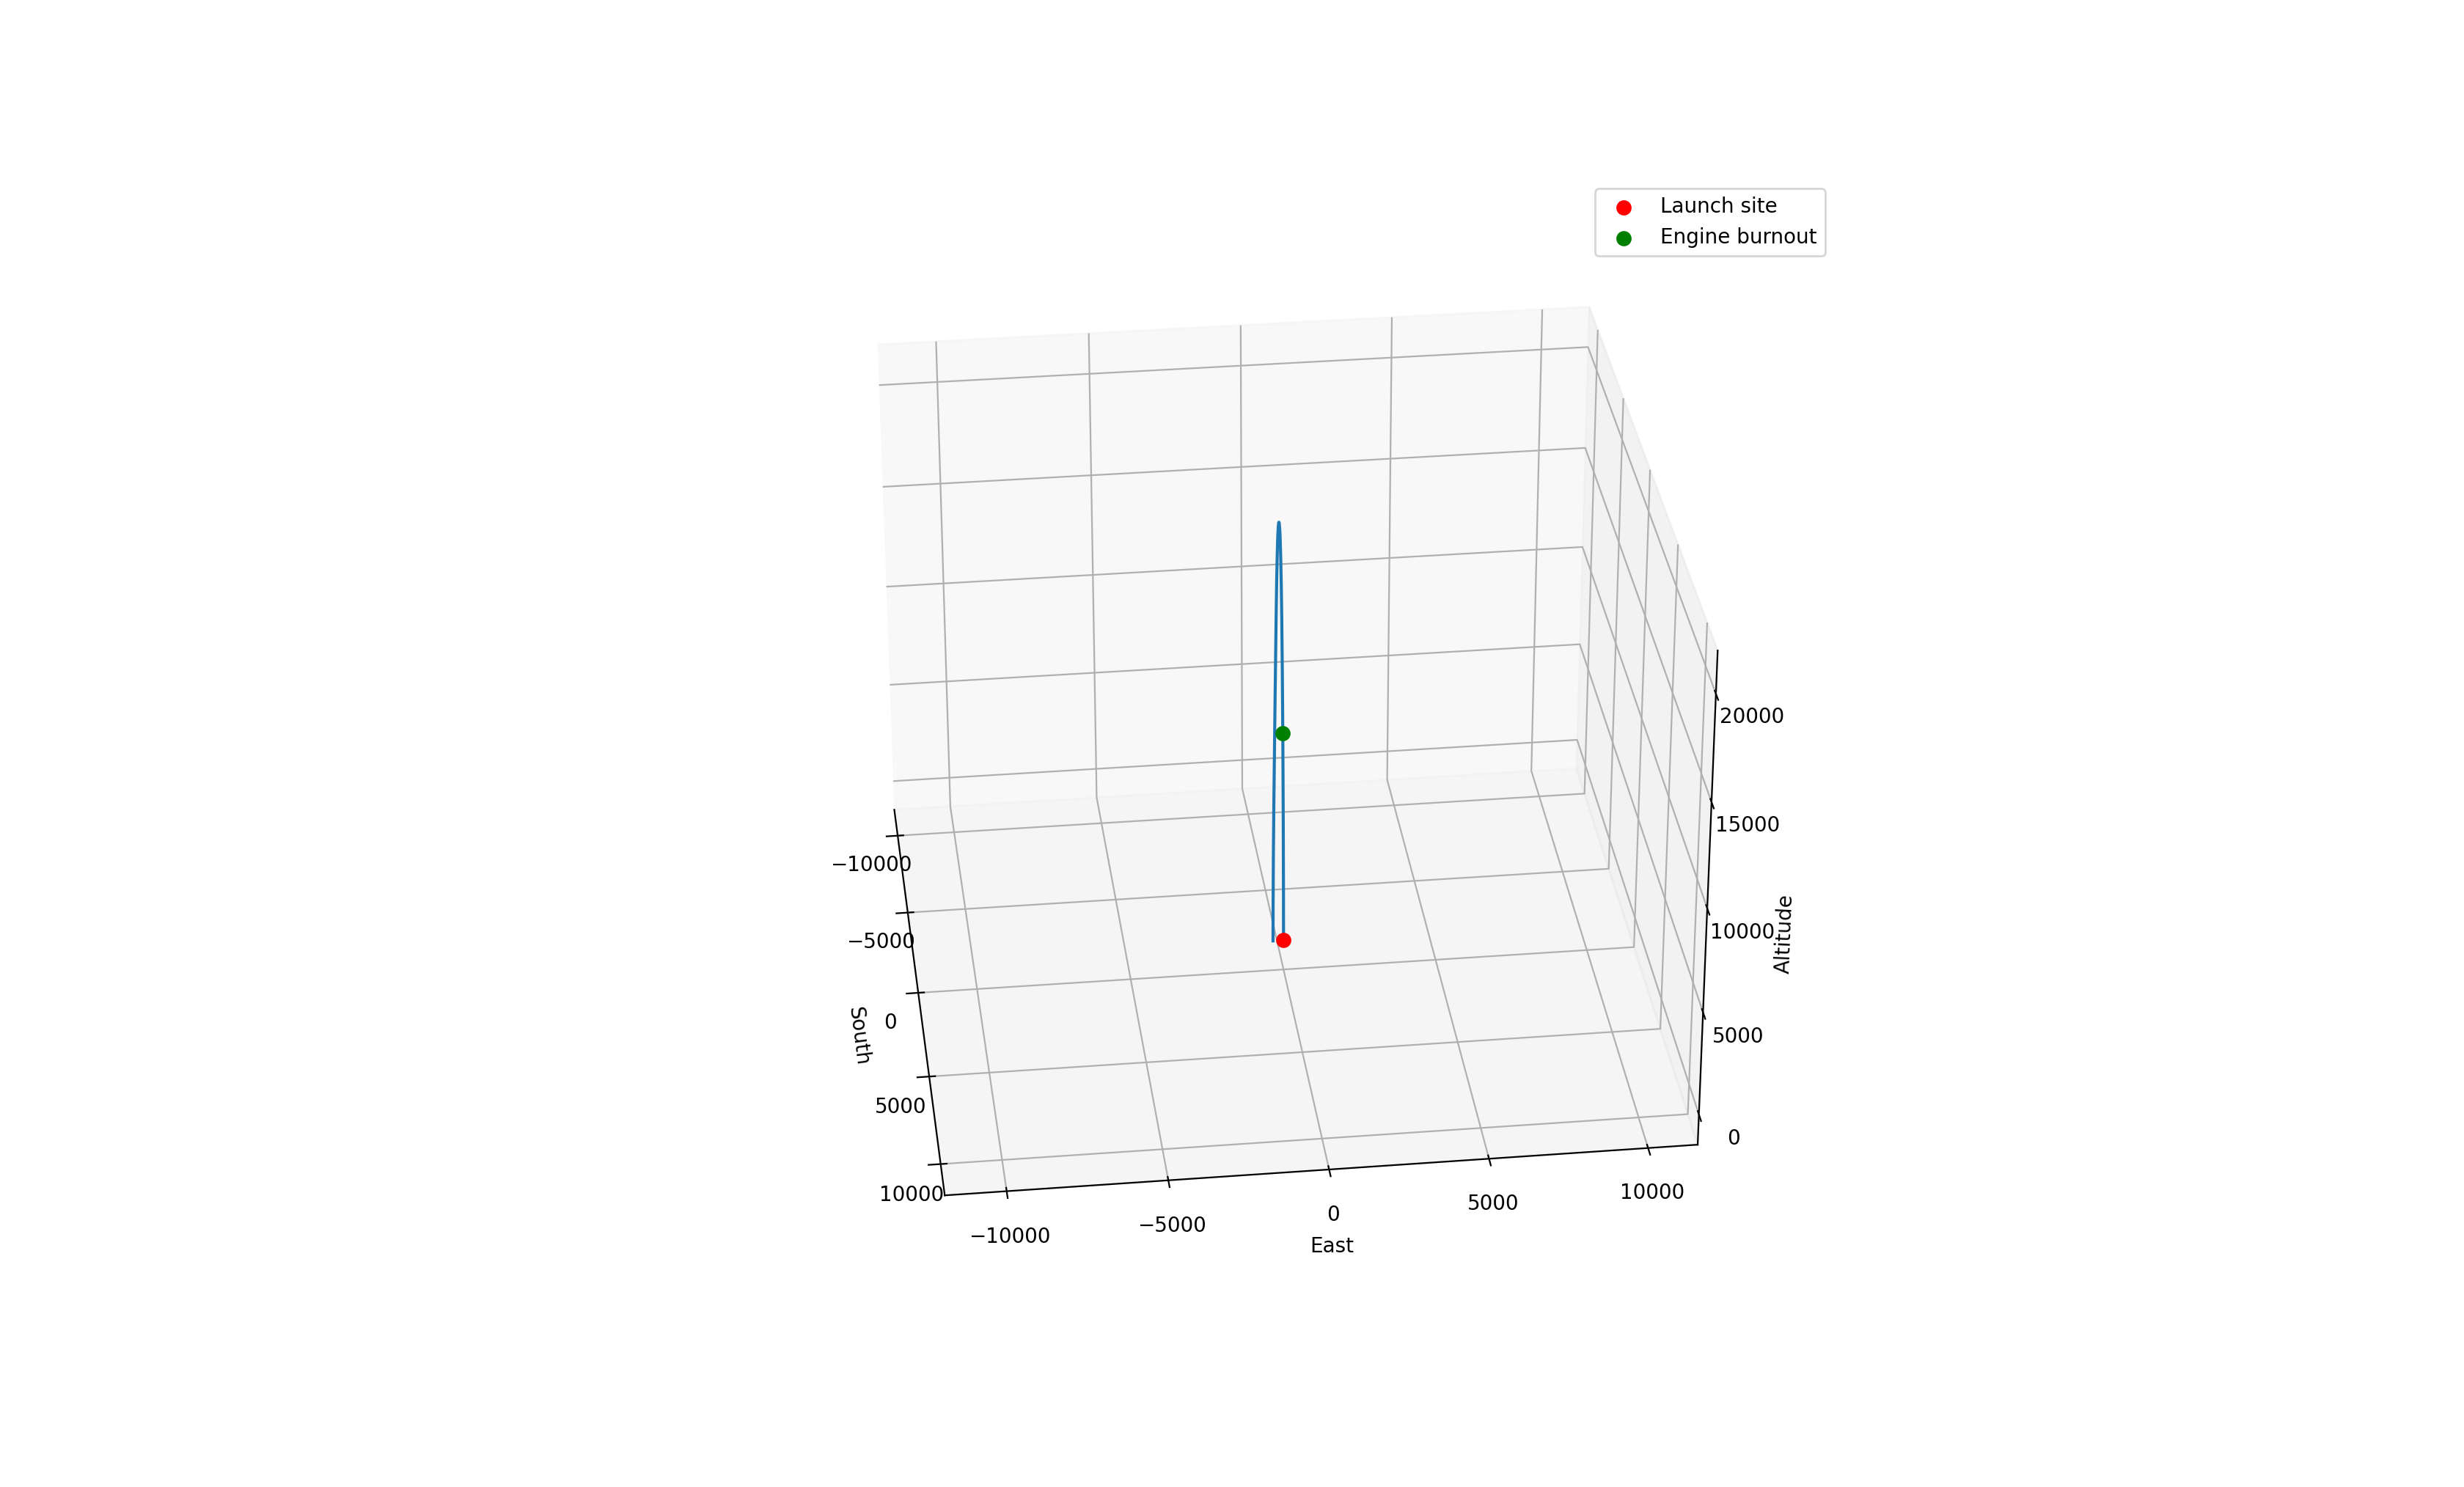
\includegraphics[width=0.85\textwidth]{images/example1.png}
    \end{frame}
    \begin{frame}
        \frametitle{Nominal Flight 1}
        \framesubtitle{2m/s Wind and 2 degree rail angle}
        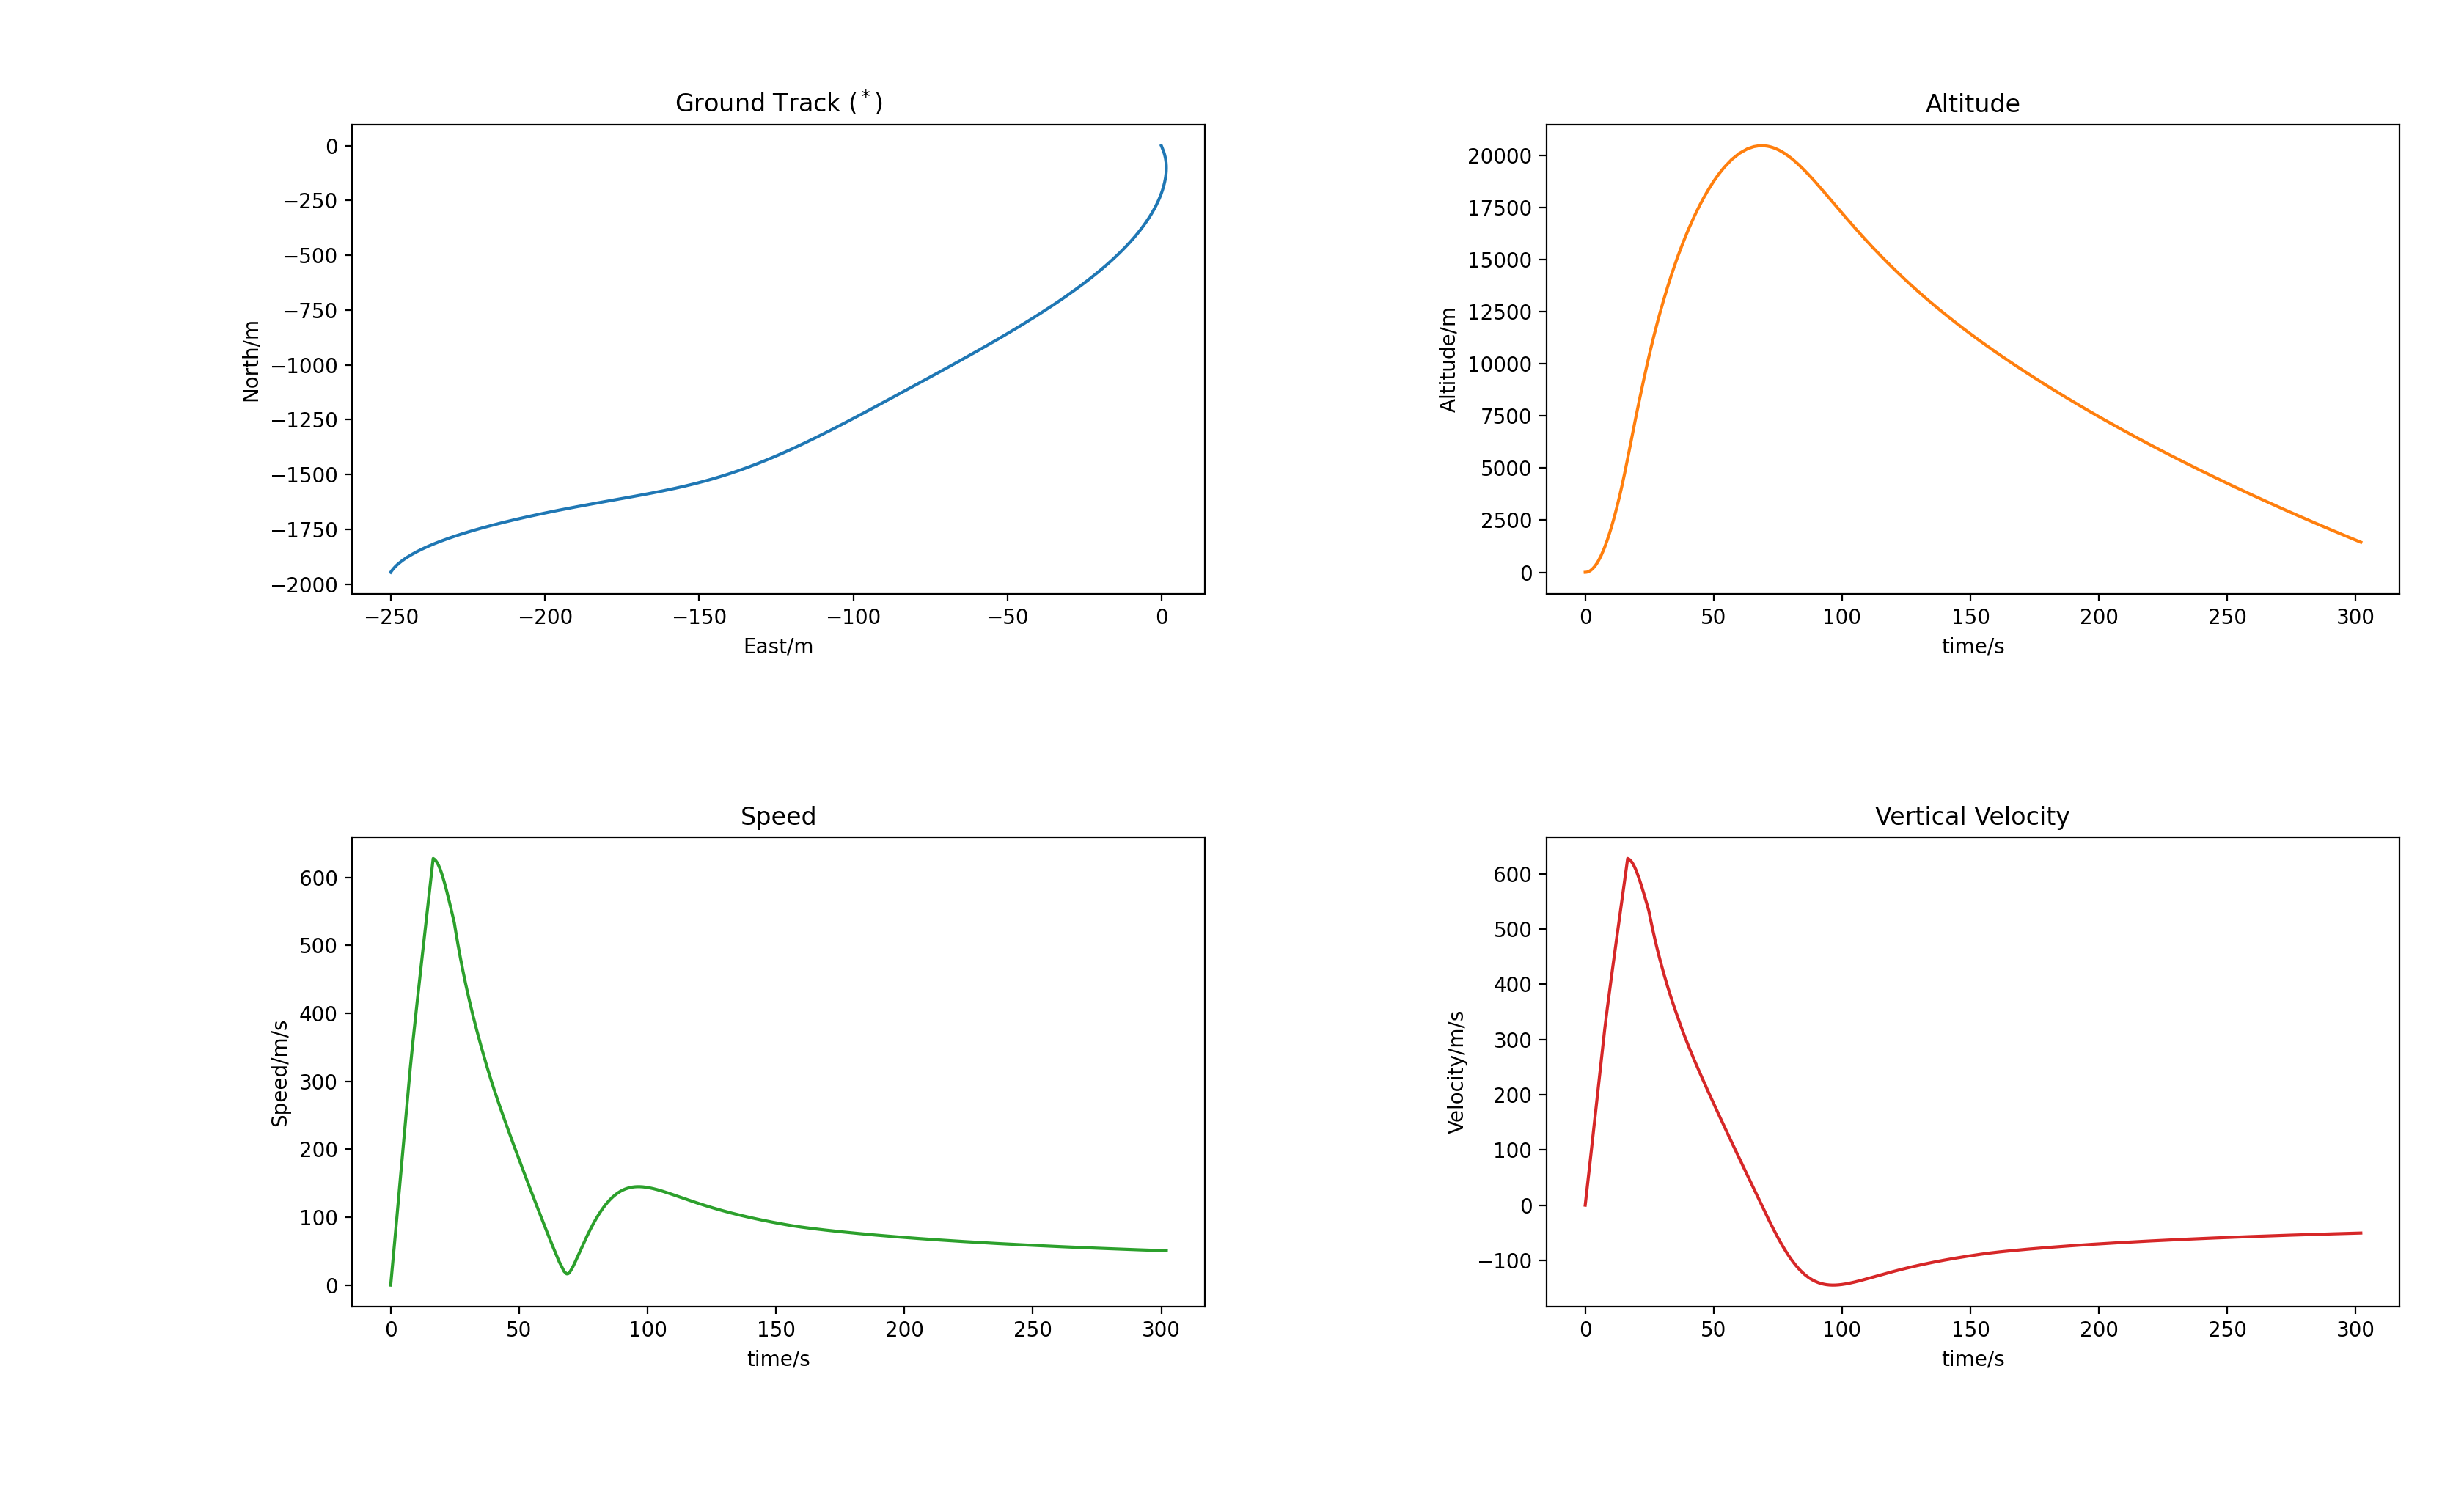
\includegraphics[width=0.85\textwidth]{images/example2.png}
    \end{frame}
    \begin{frame}
        \frametitle{Nominal Flight 1}
        \framesubtitle{2m/s Wind and 2 degree rail angle}
        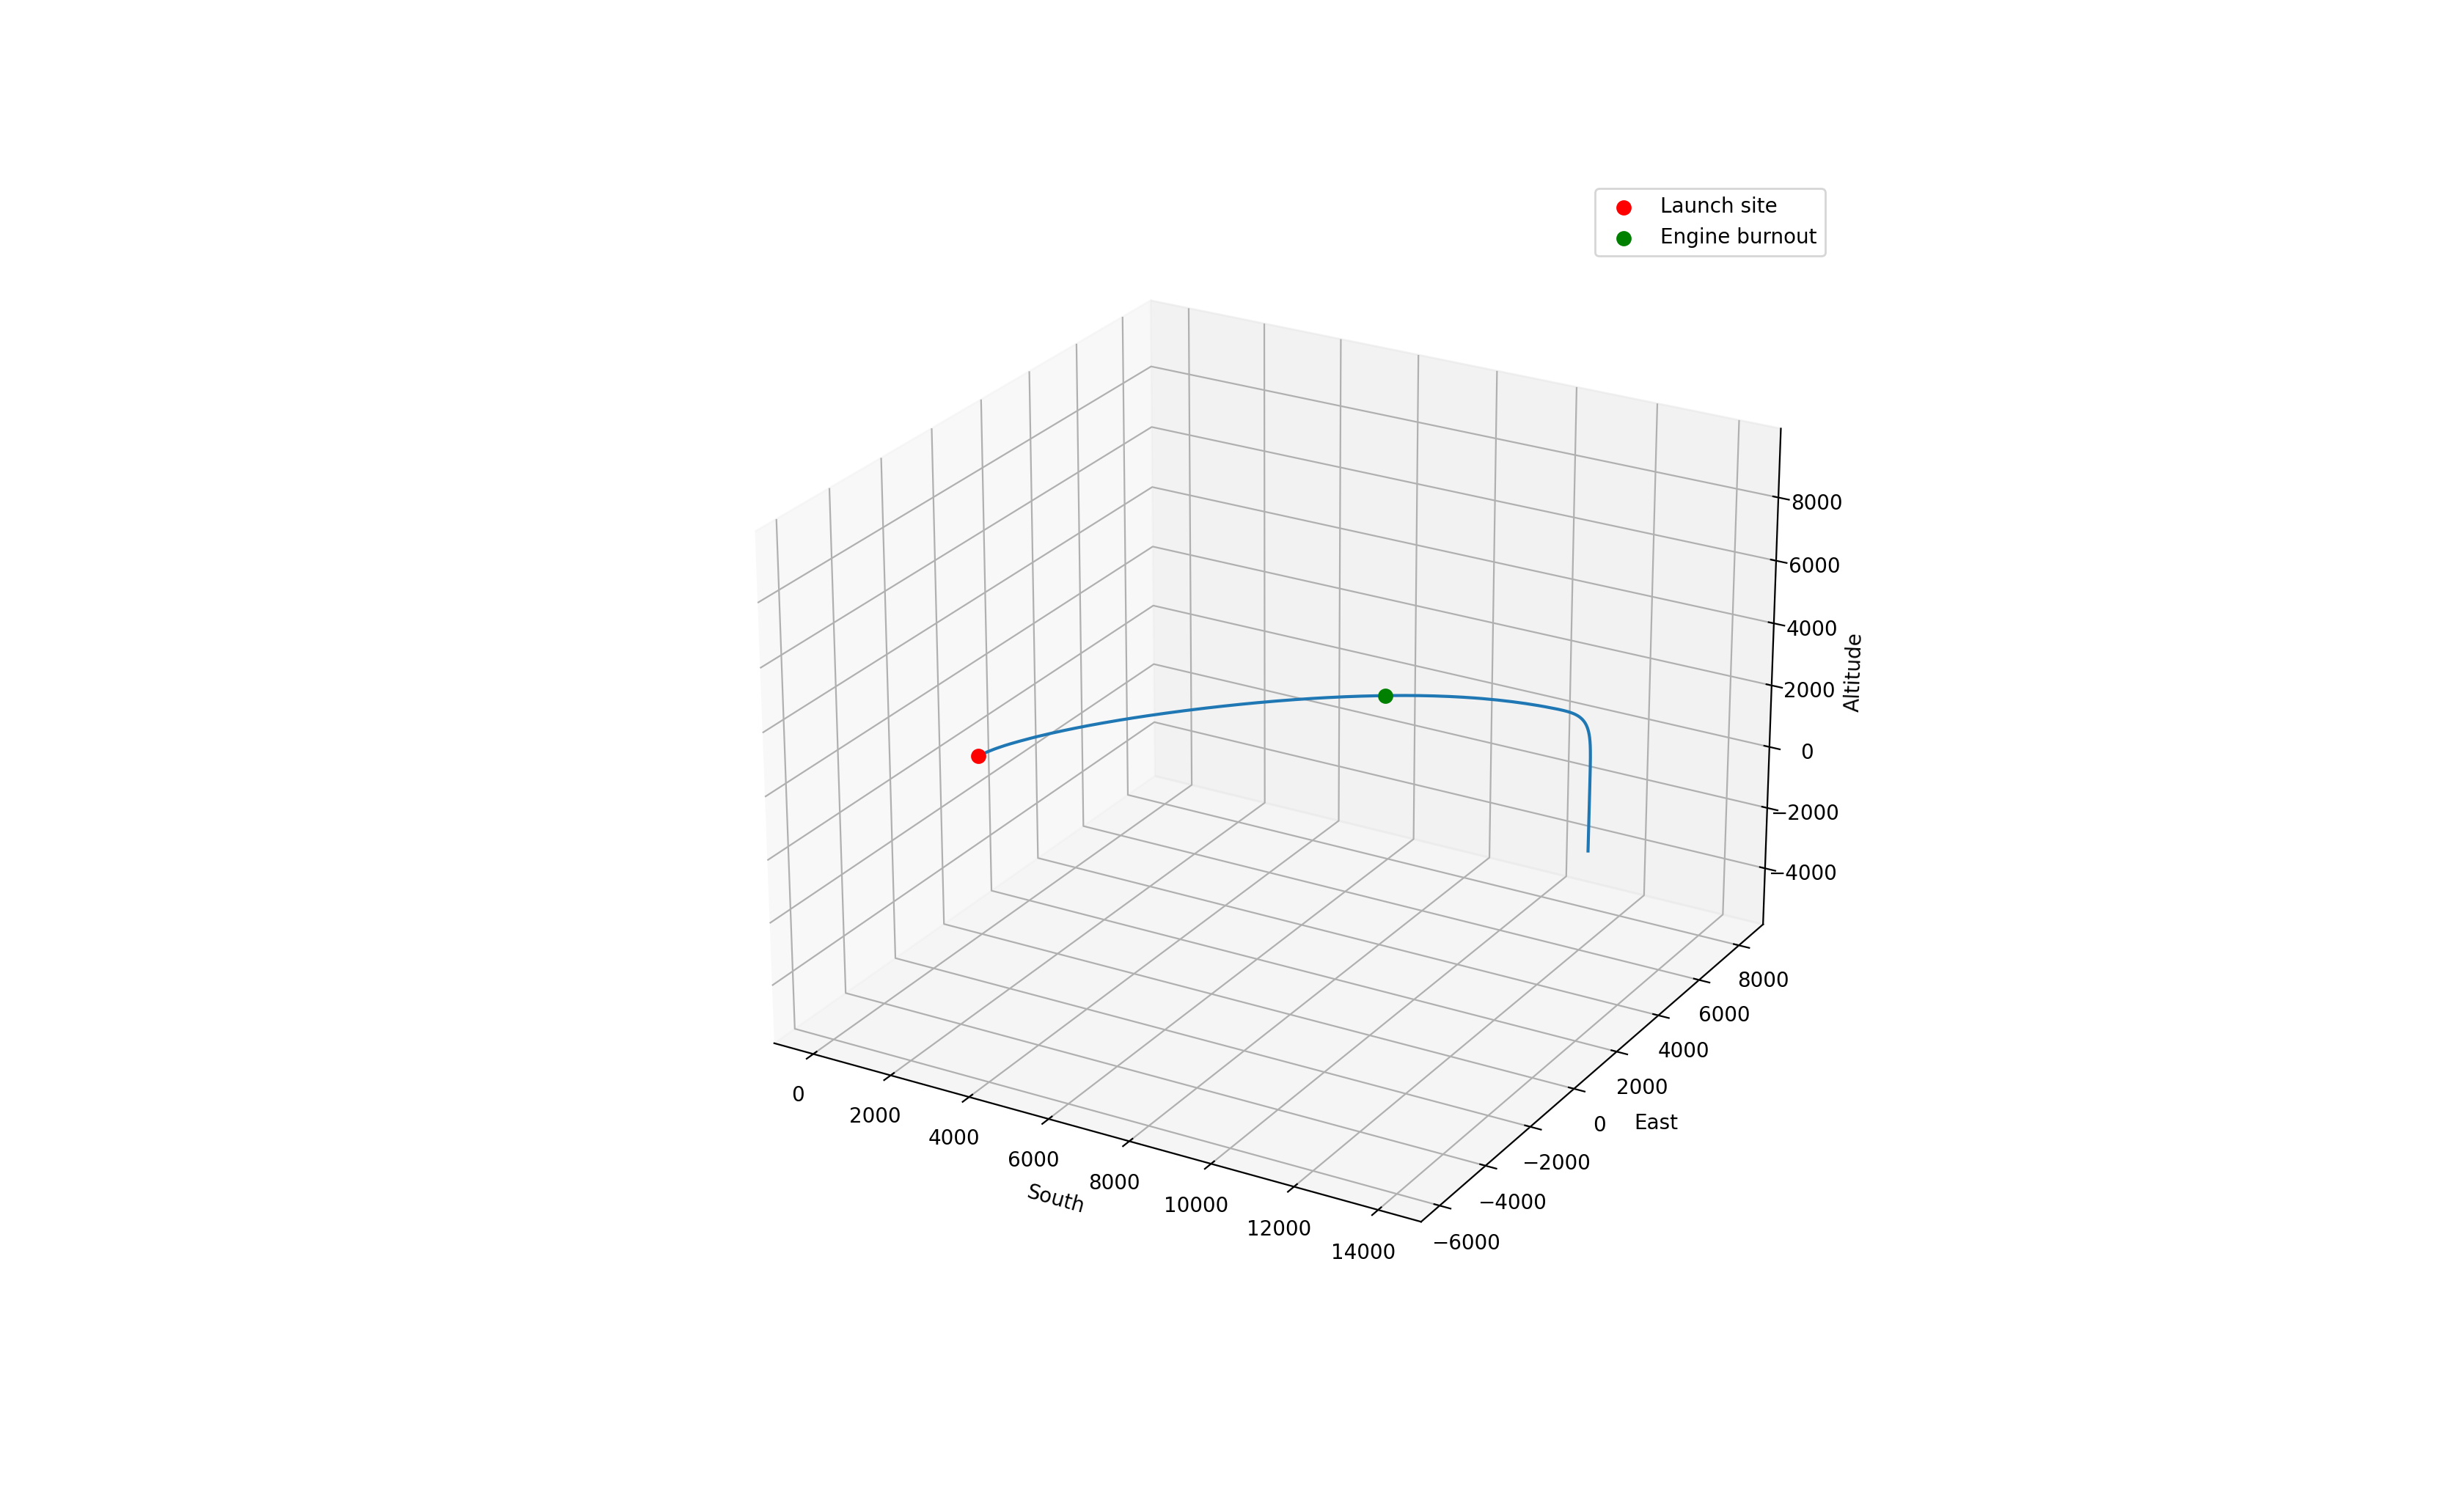
\includegraphics[width=0.85\textwidth]{images/example3.png}
    \end{frame}
    \begin{frame}
        \frametitle{Nominal Flight 2}
        \framesubtitle{No wild or rail angle, jaggedness from automatic step size reduction (note the scale on the downrange is $1\times10^{-11}$)}
        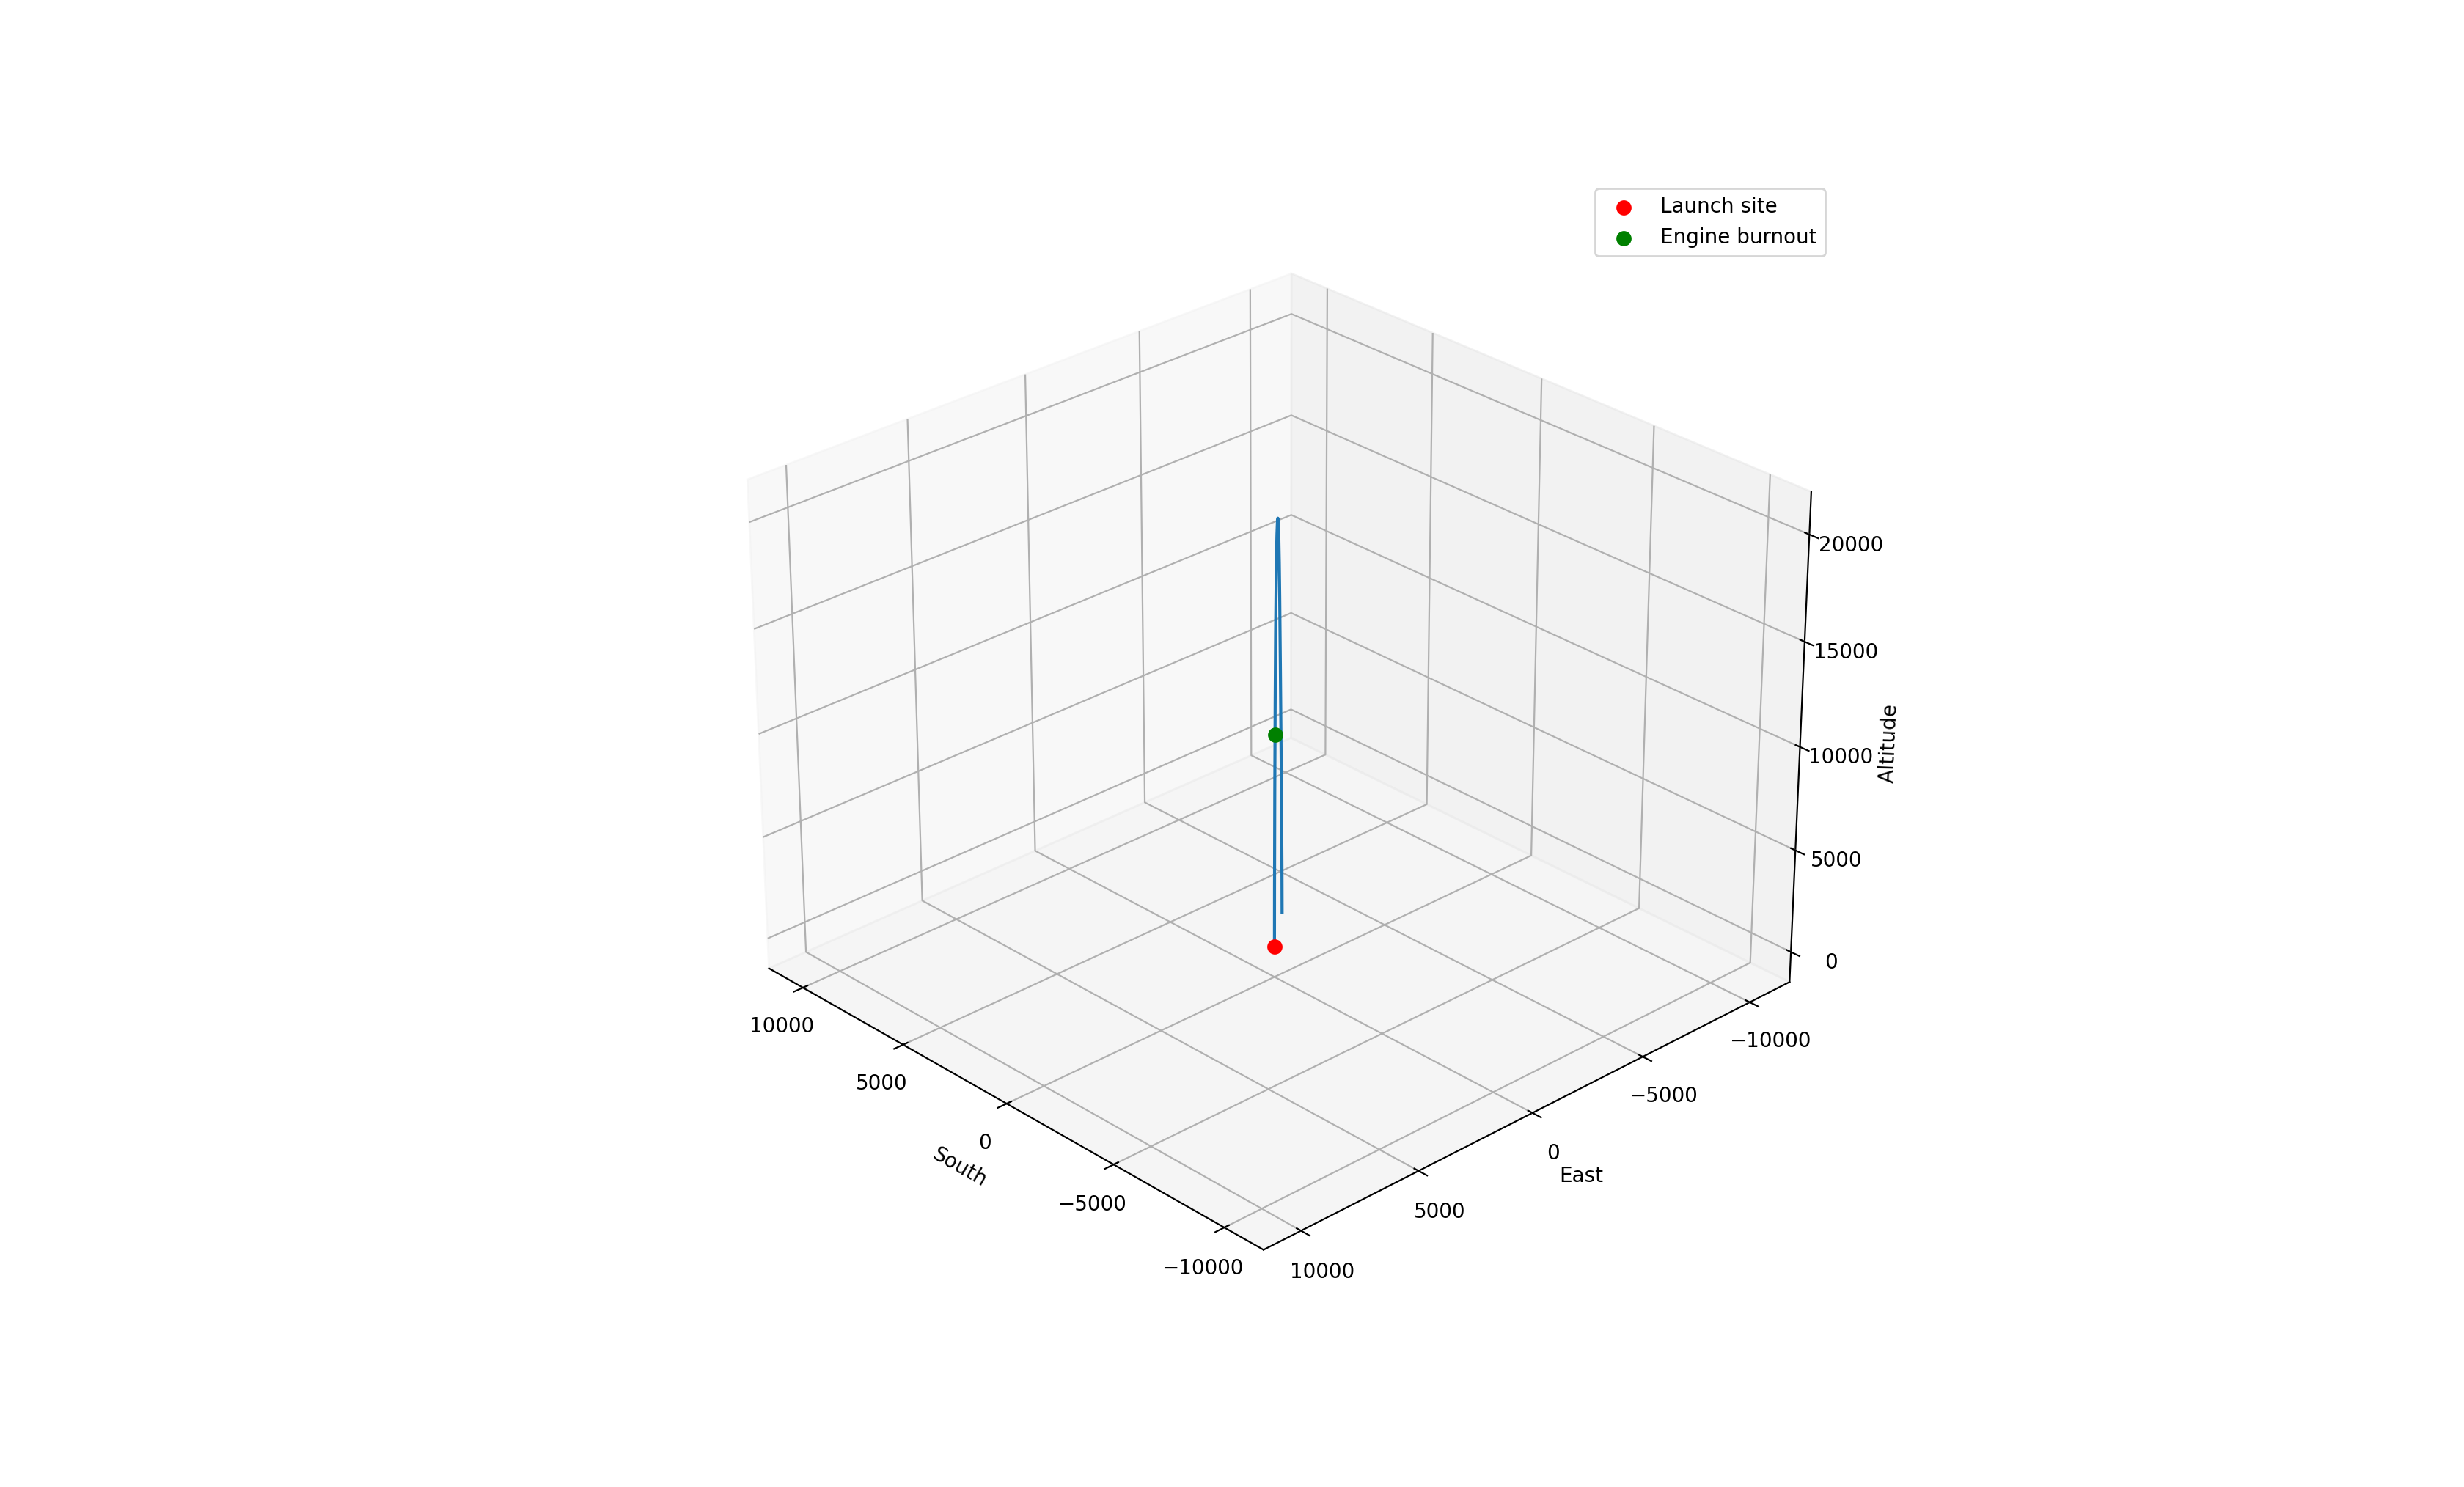
\includegraphics[width=0.85\textwidth]{images/example1a.png}
    \end{frame}
    \begin{frame}
        \frametitle{Nominal Flight 2}
        \framesubtitle{No wild or rail angle, jaggedness from automatic step size reduction (note the scale on the downrange is $1\times10^{-11}$)}
        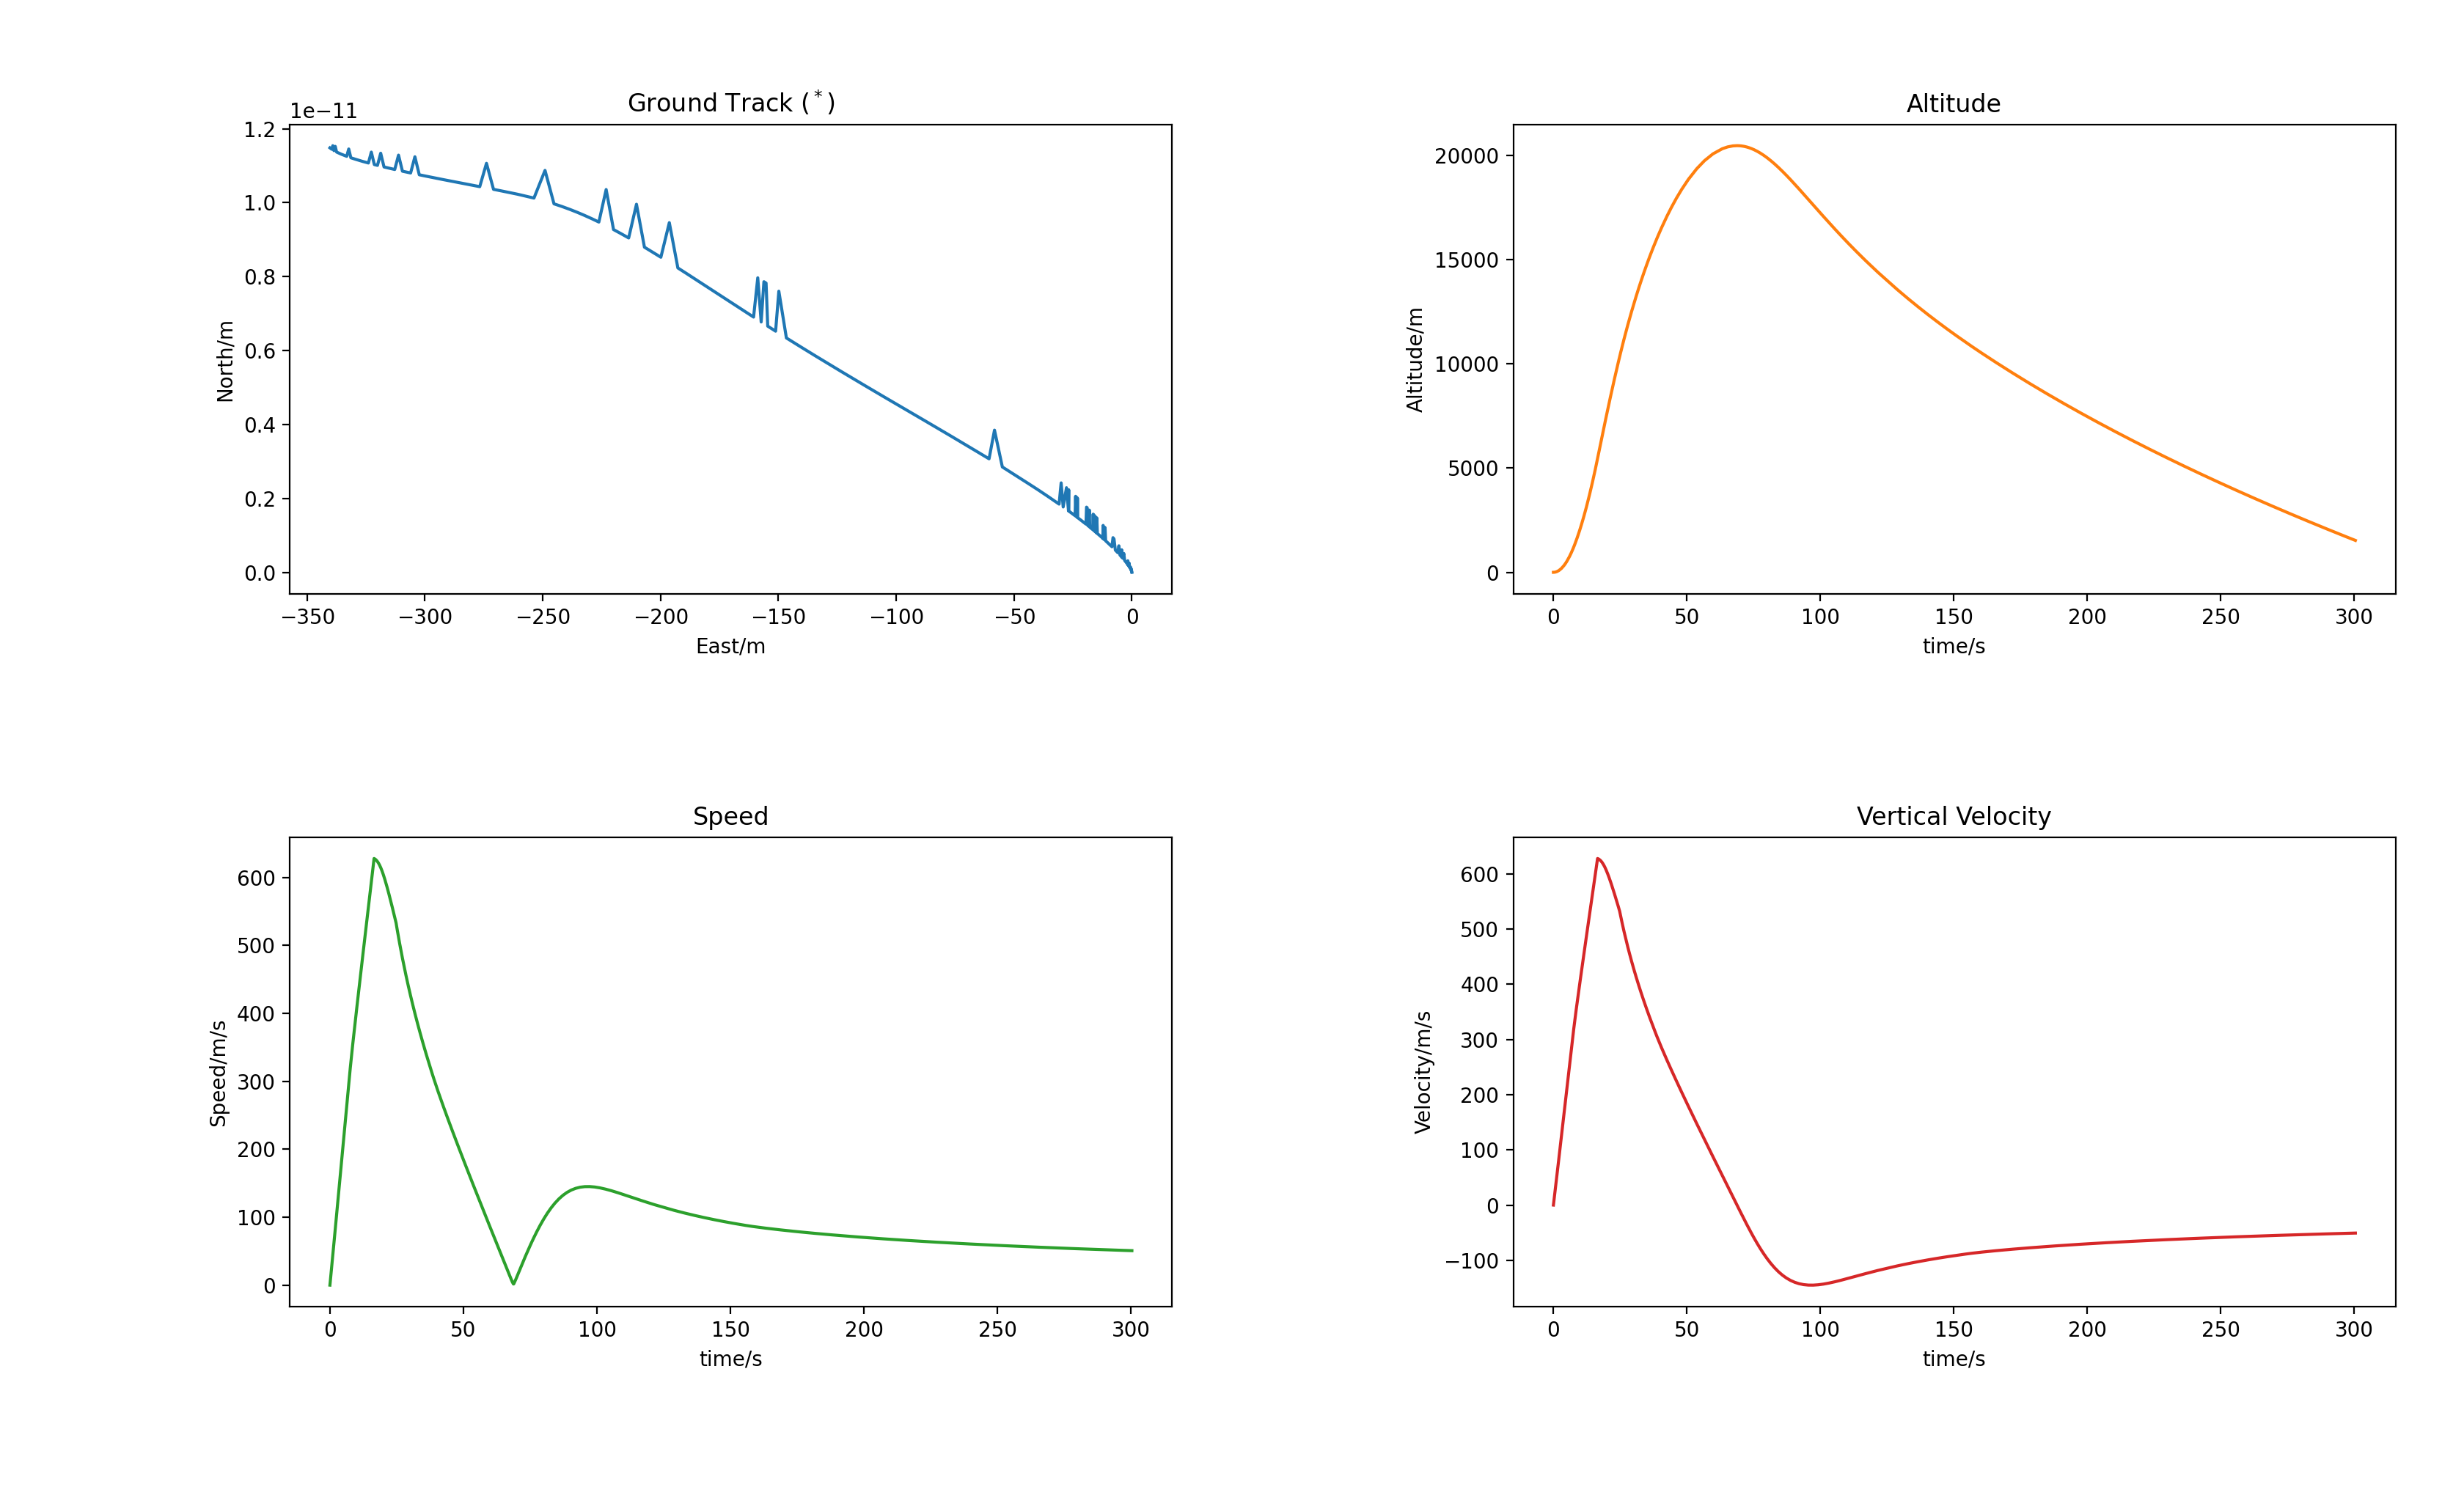
\includegraphics[width=0.85\textwidth]{images/example2a.png}
    \end{frame}
    \begin{frame}
        \frametitle{Nominal Flight 2}
        \framesubtitle{No wild or rail angle, jaggedness from automatic step size reduction (note the scale on the downrange is $1\times10^{-11}$)}
        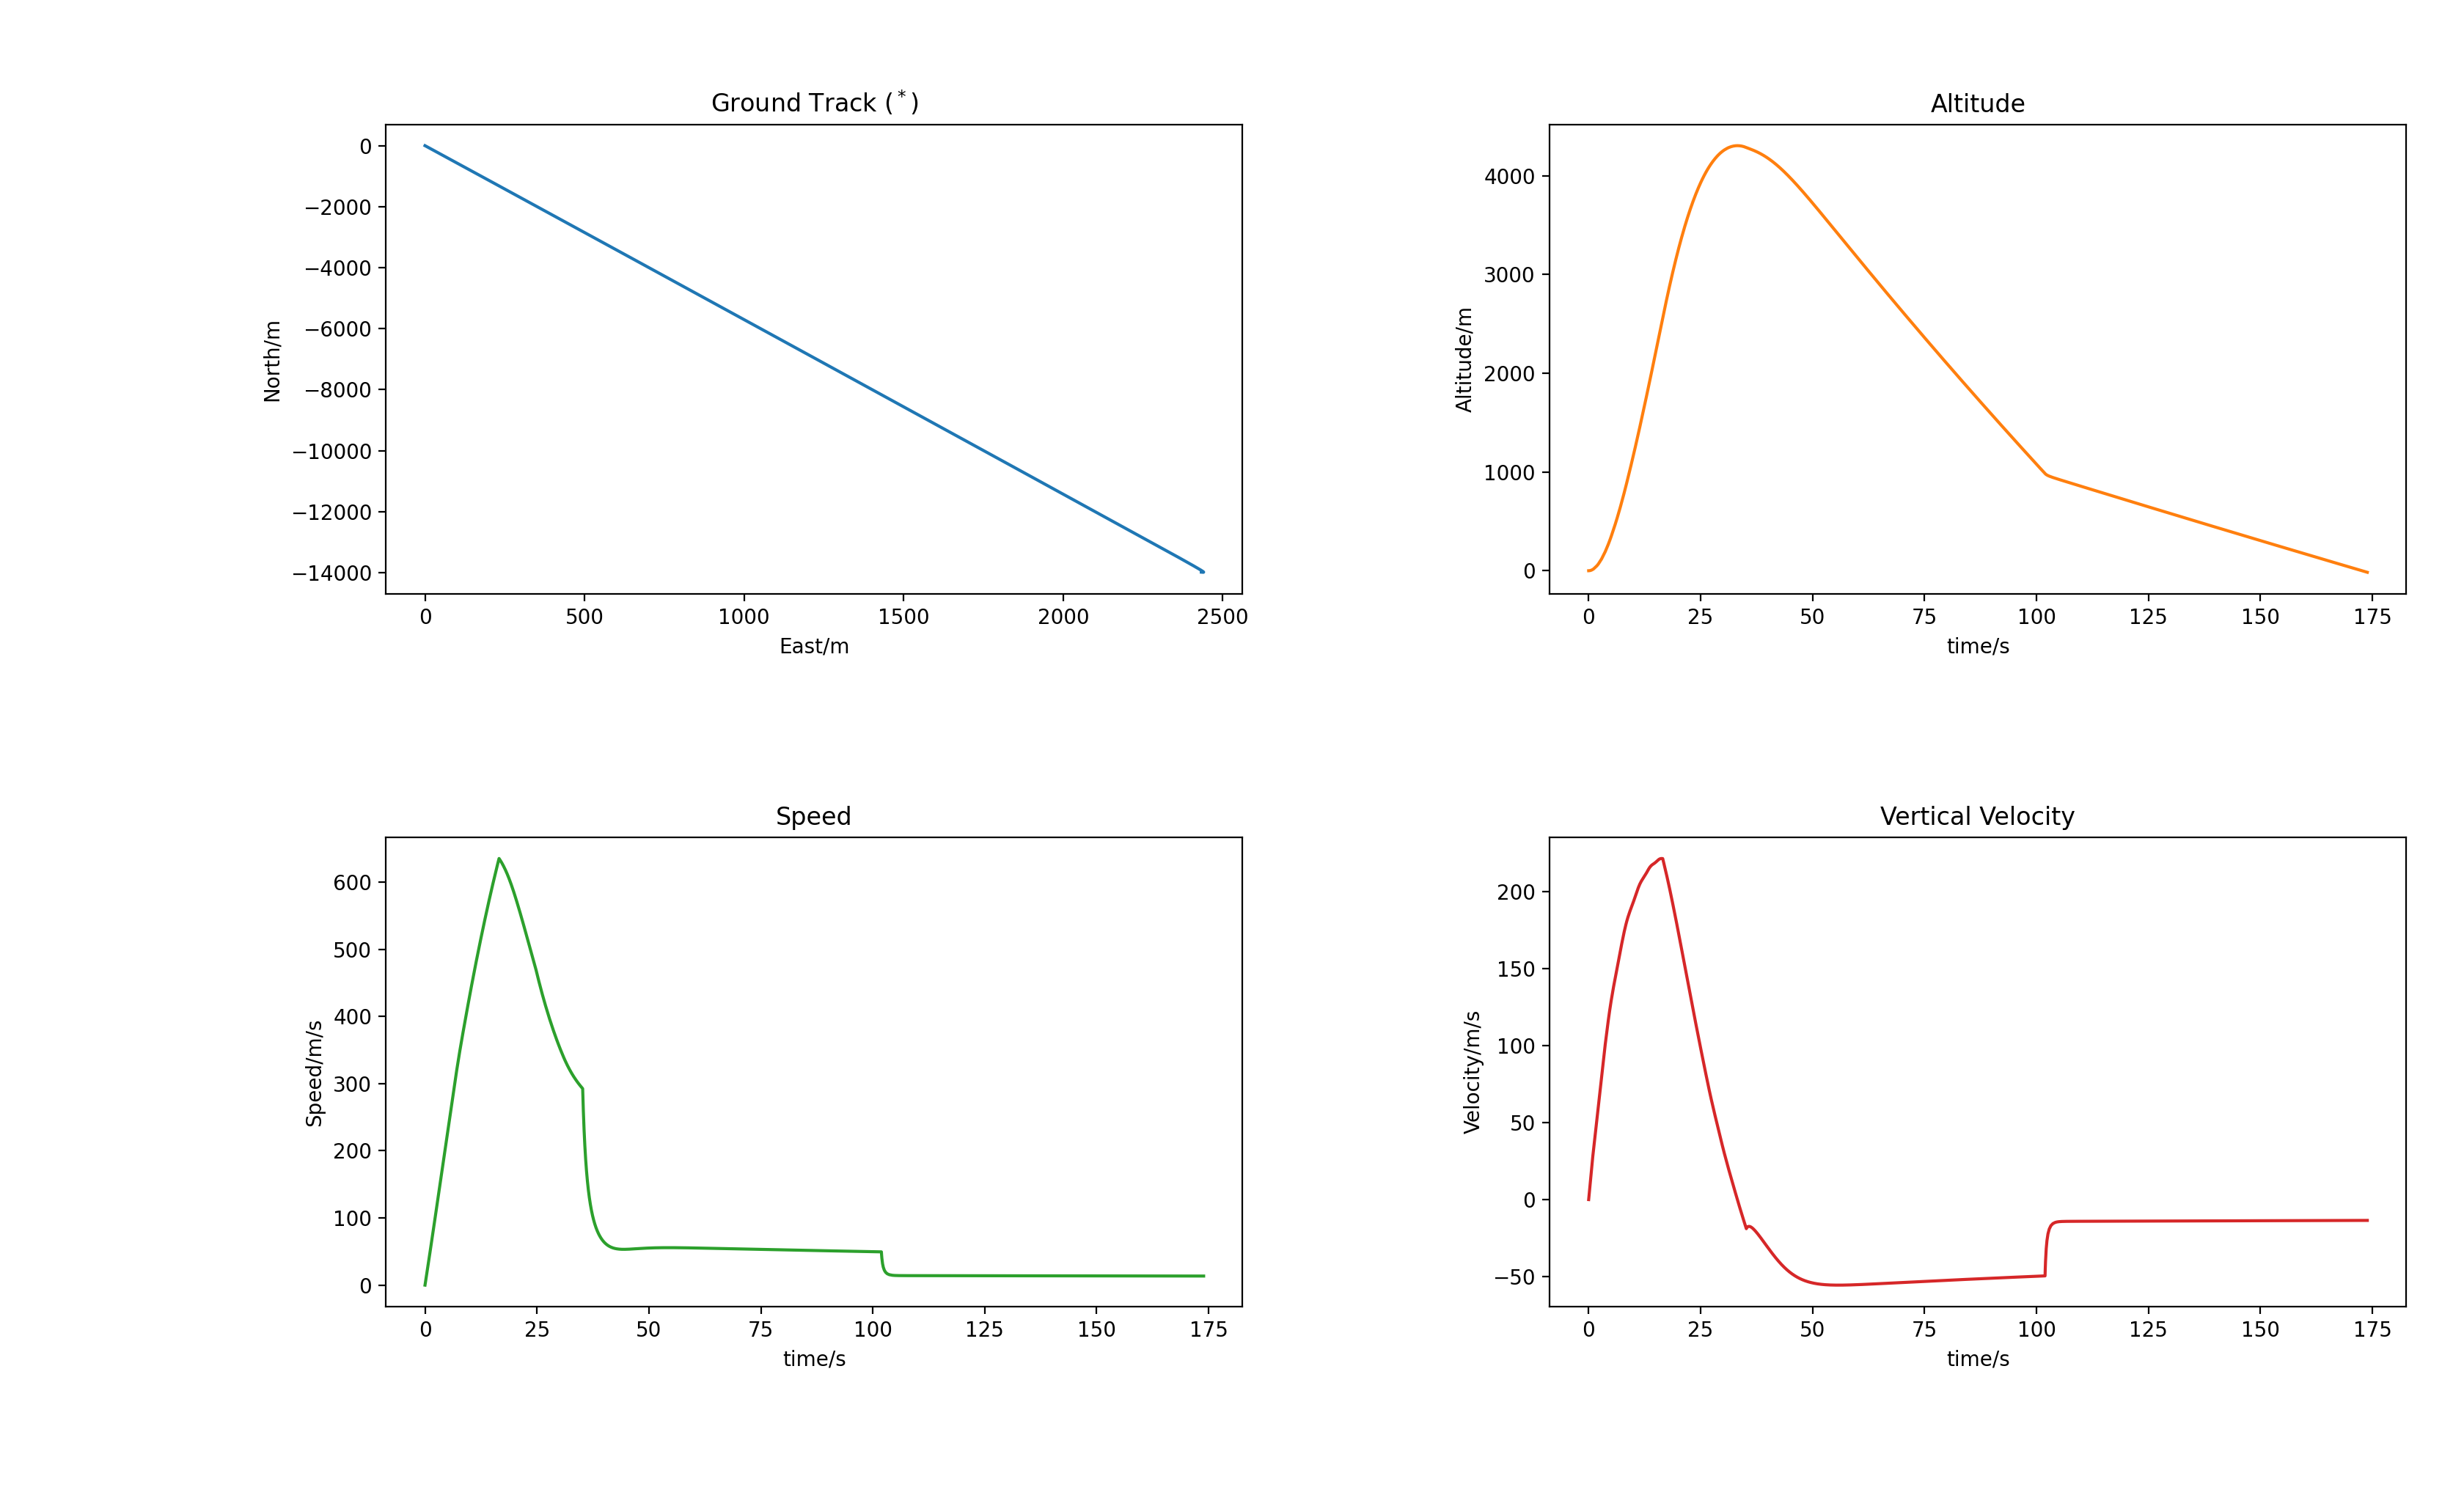
\includegraphics[width=0.85\textwidth]{images/example3a.png}
    \end{frame}
    \begin{frame}
        \frametitle{Nominal Flight 3}
        \framesubtitle{45 degree rail angle}
        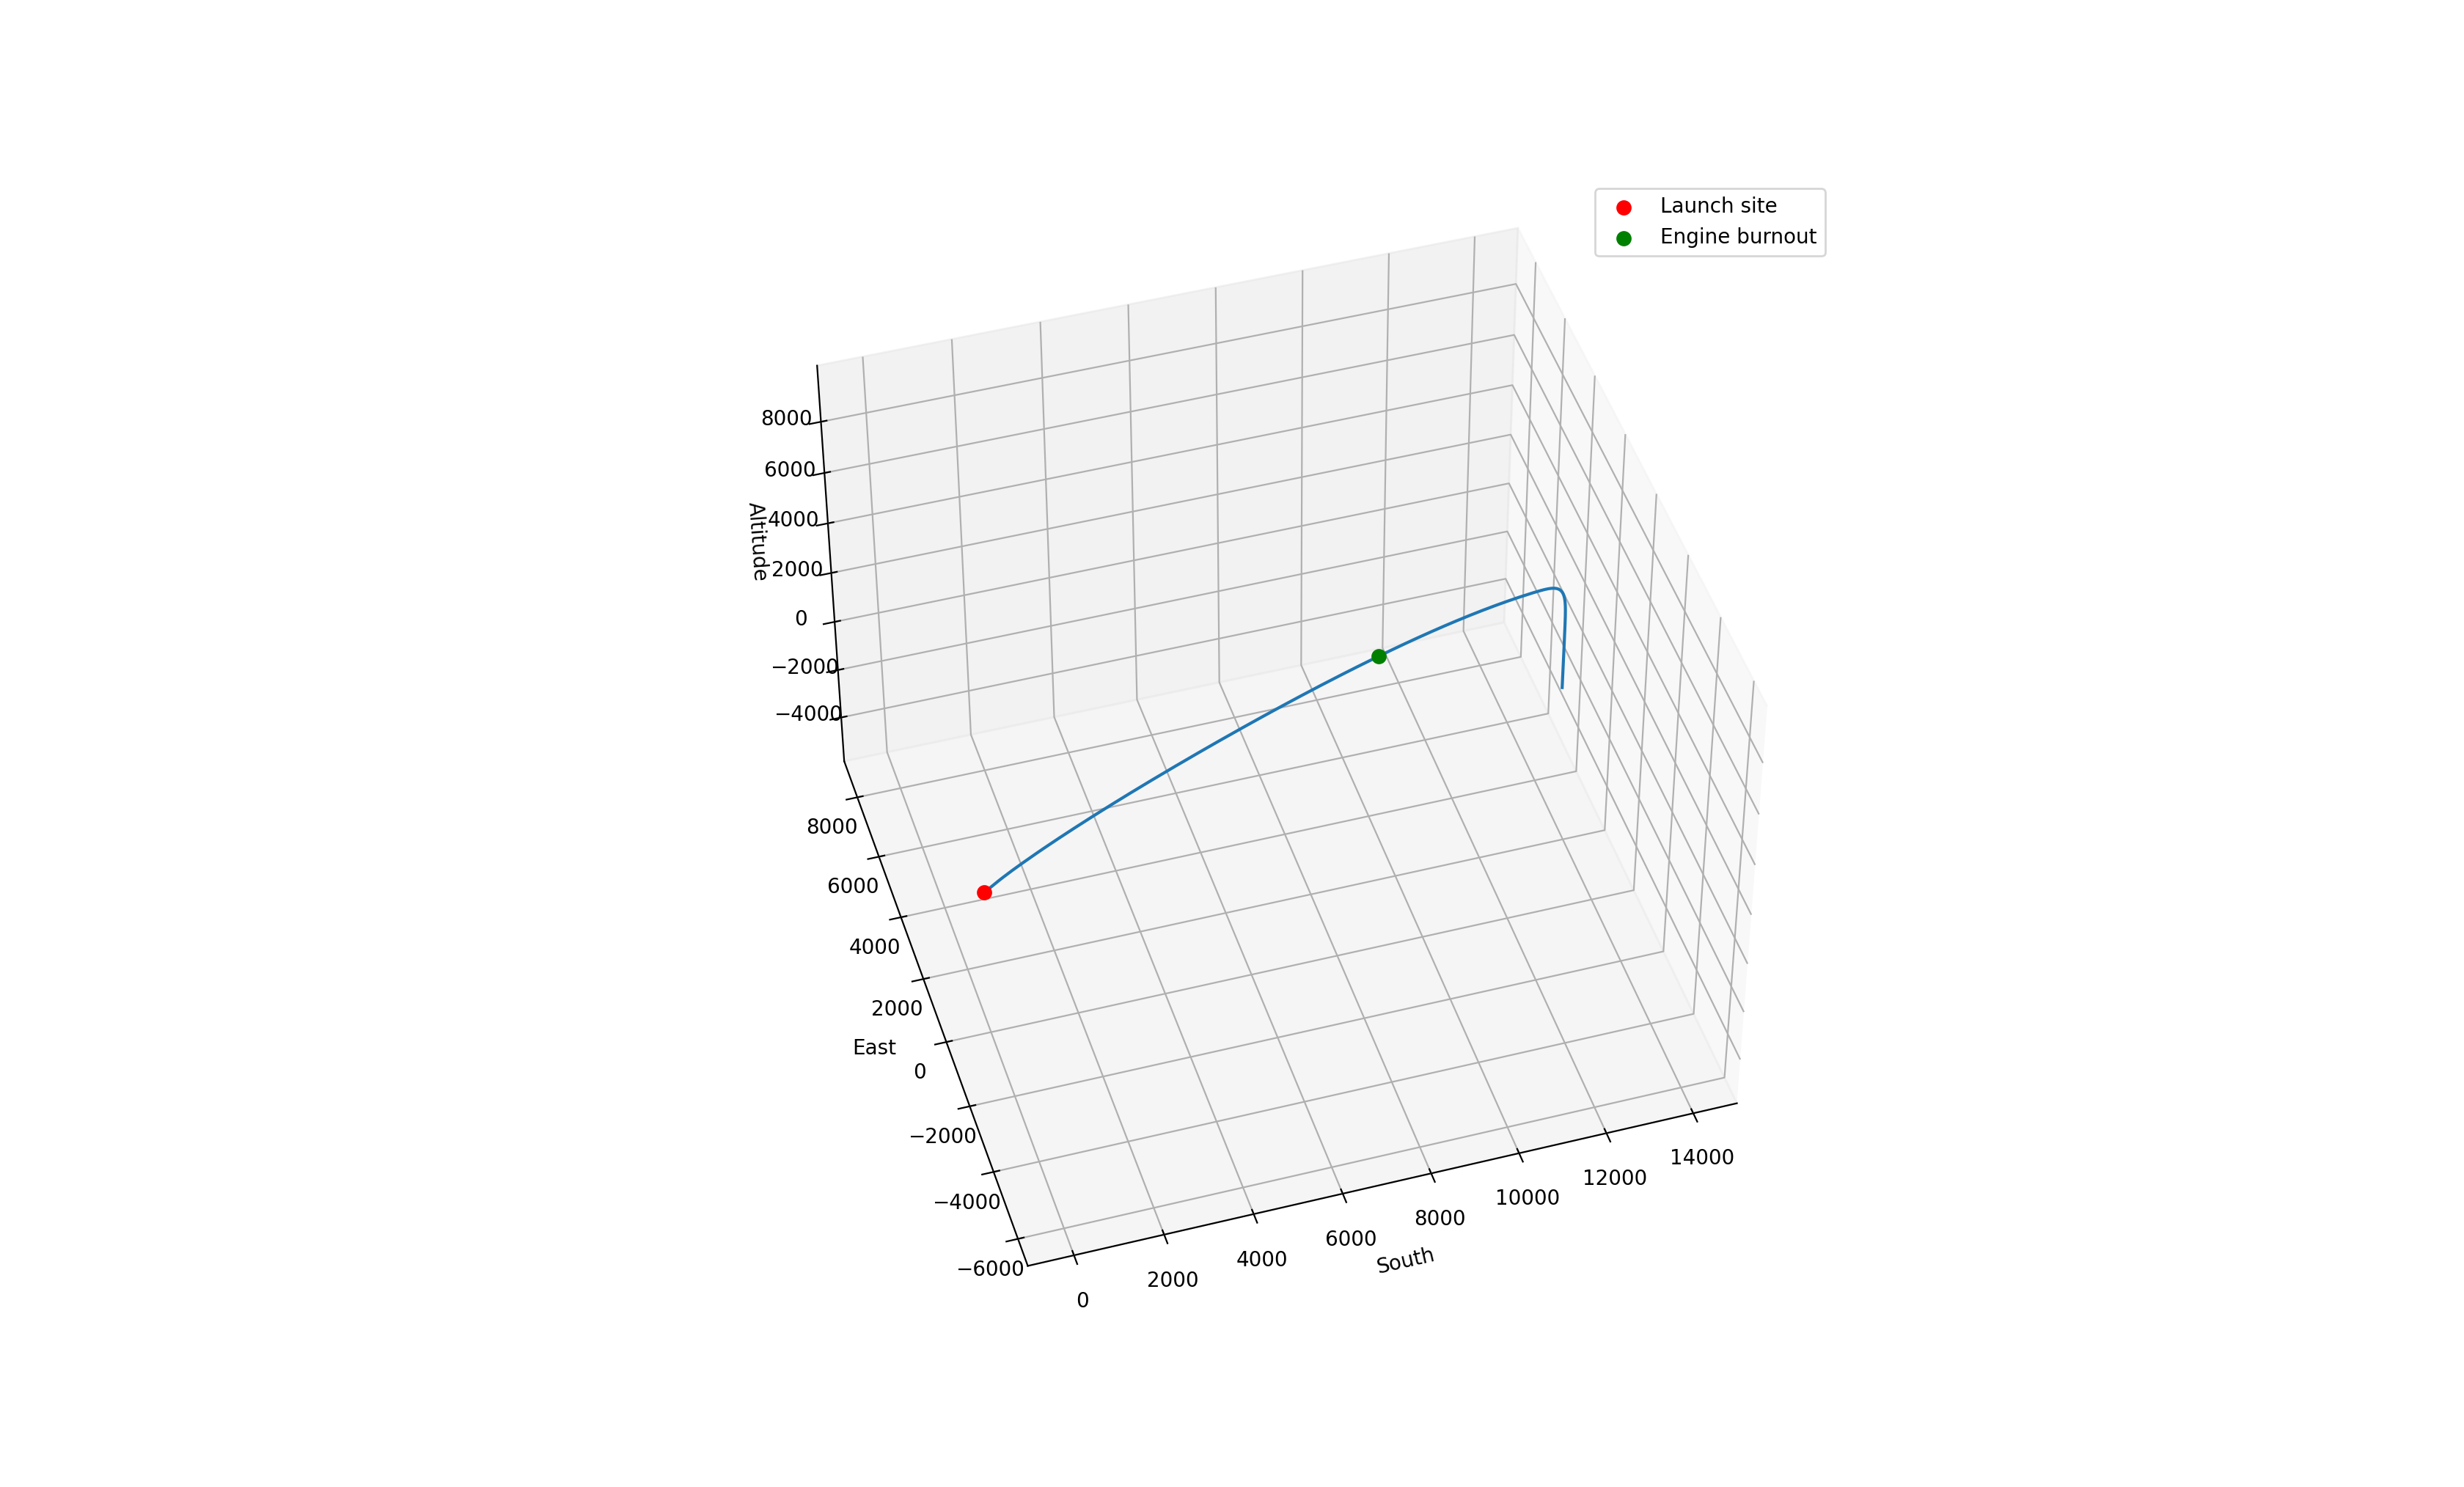
\includegraphics[width=0.85\textwidth]{images/example1b.png}
    \end{frame}
    \begin{frame}
        \frametitle{Nominal Flight 3}
        \framesubtitle{45 degree rail angle}
        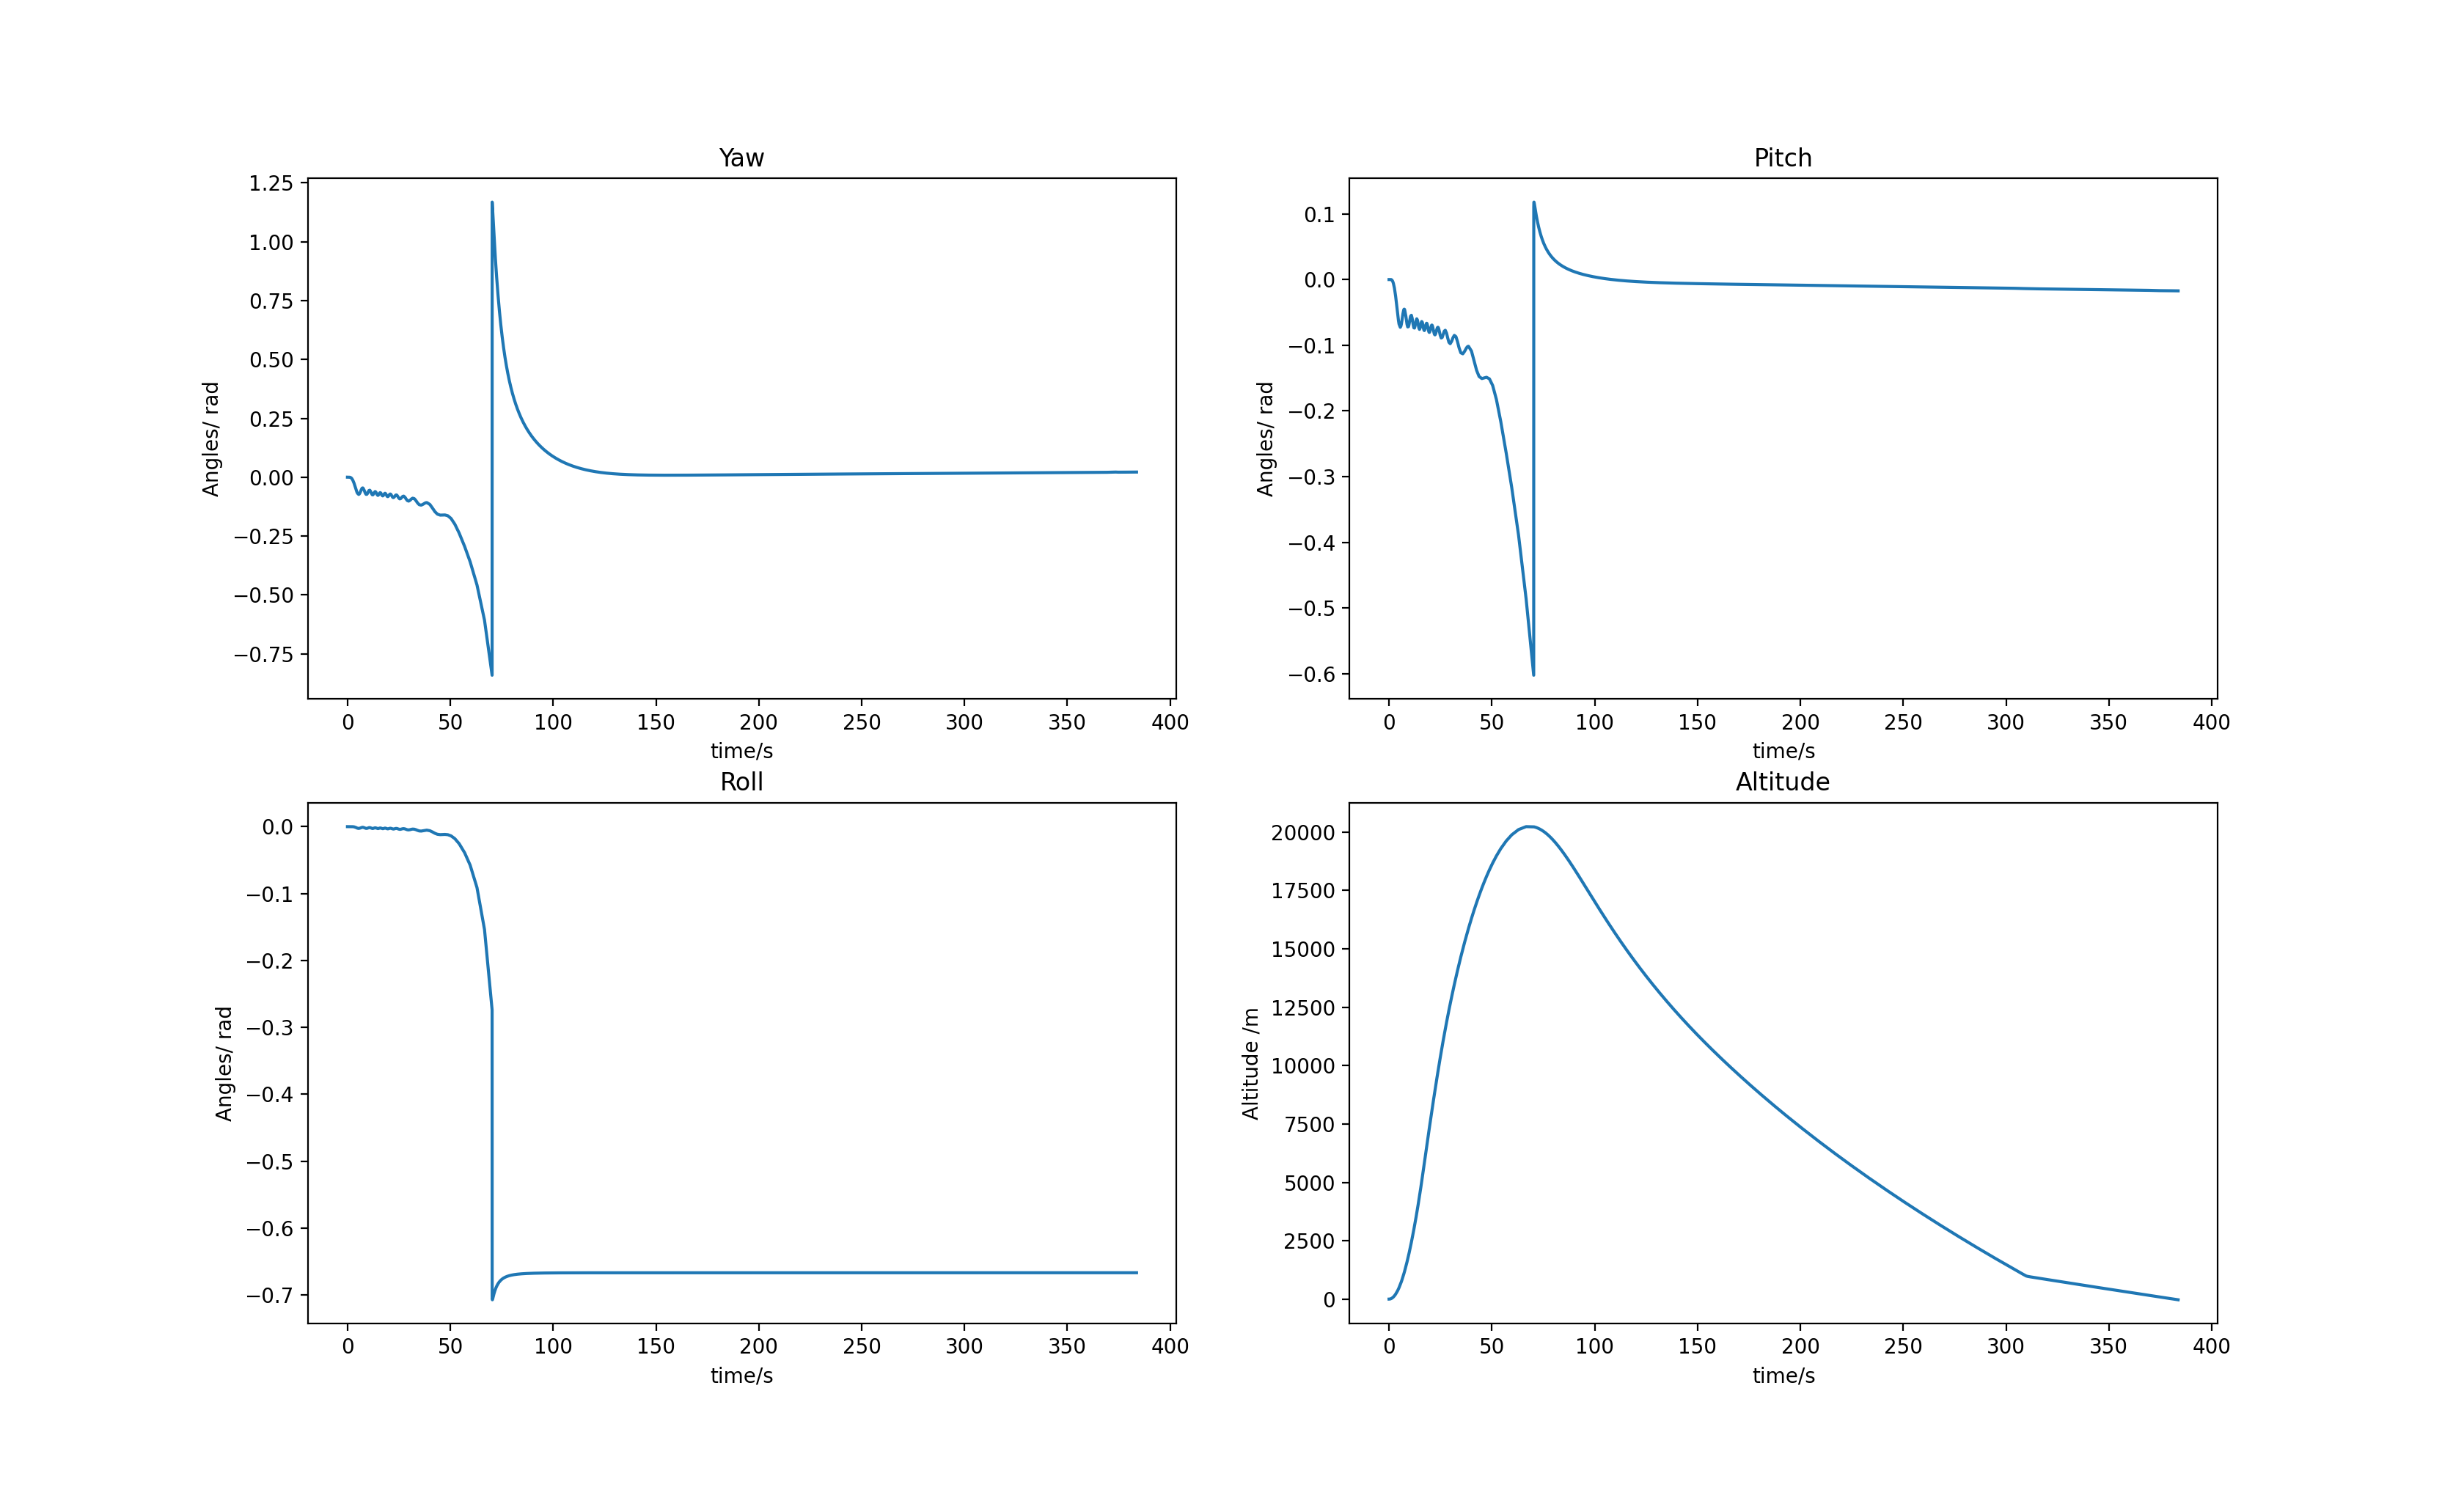
\includegraphics[width=0.85\textwidth]{images/example2b.png}
    \end{frame}
    \begin{frame}
        \frametitle{Nominal Flight 3}
        \framesubtitle{45 degree rail angle}
        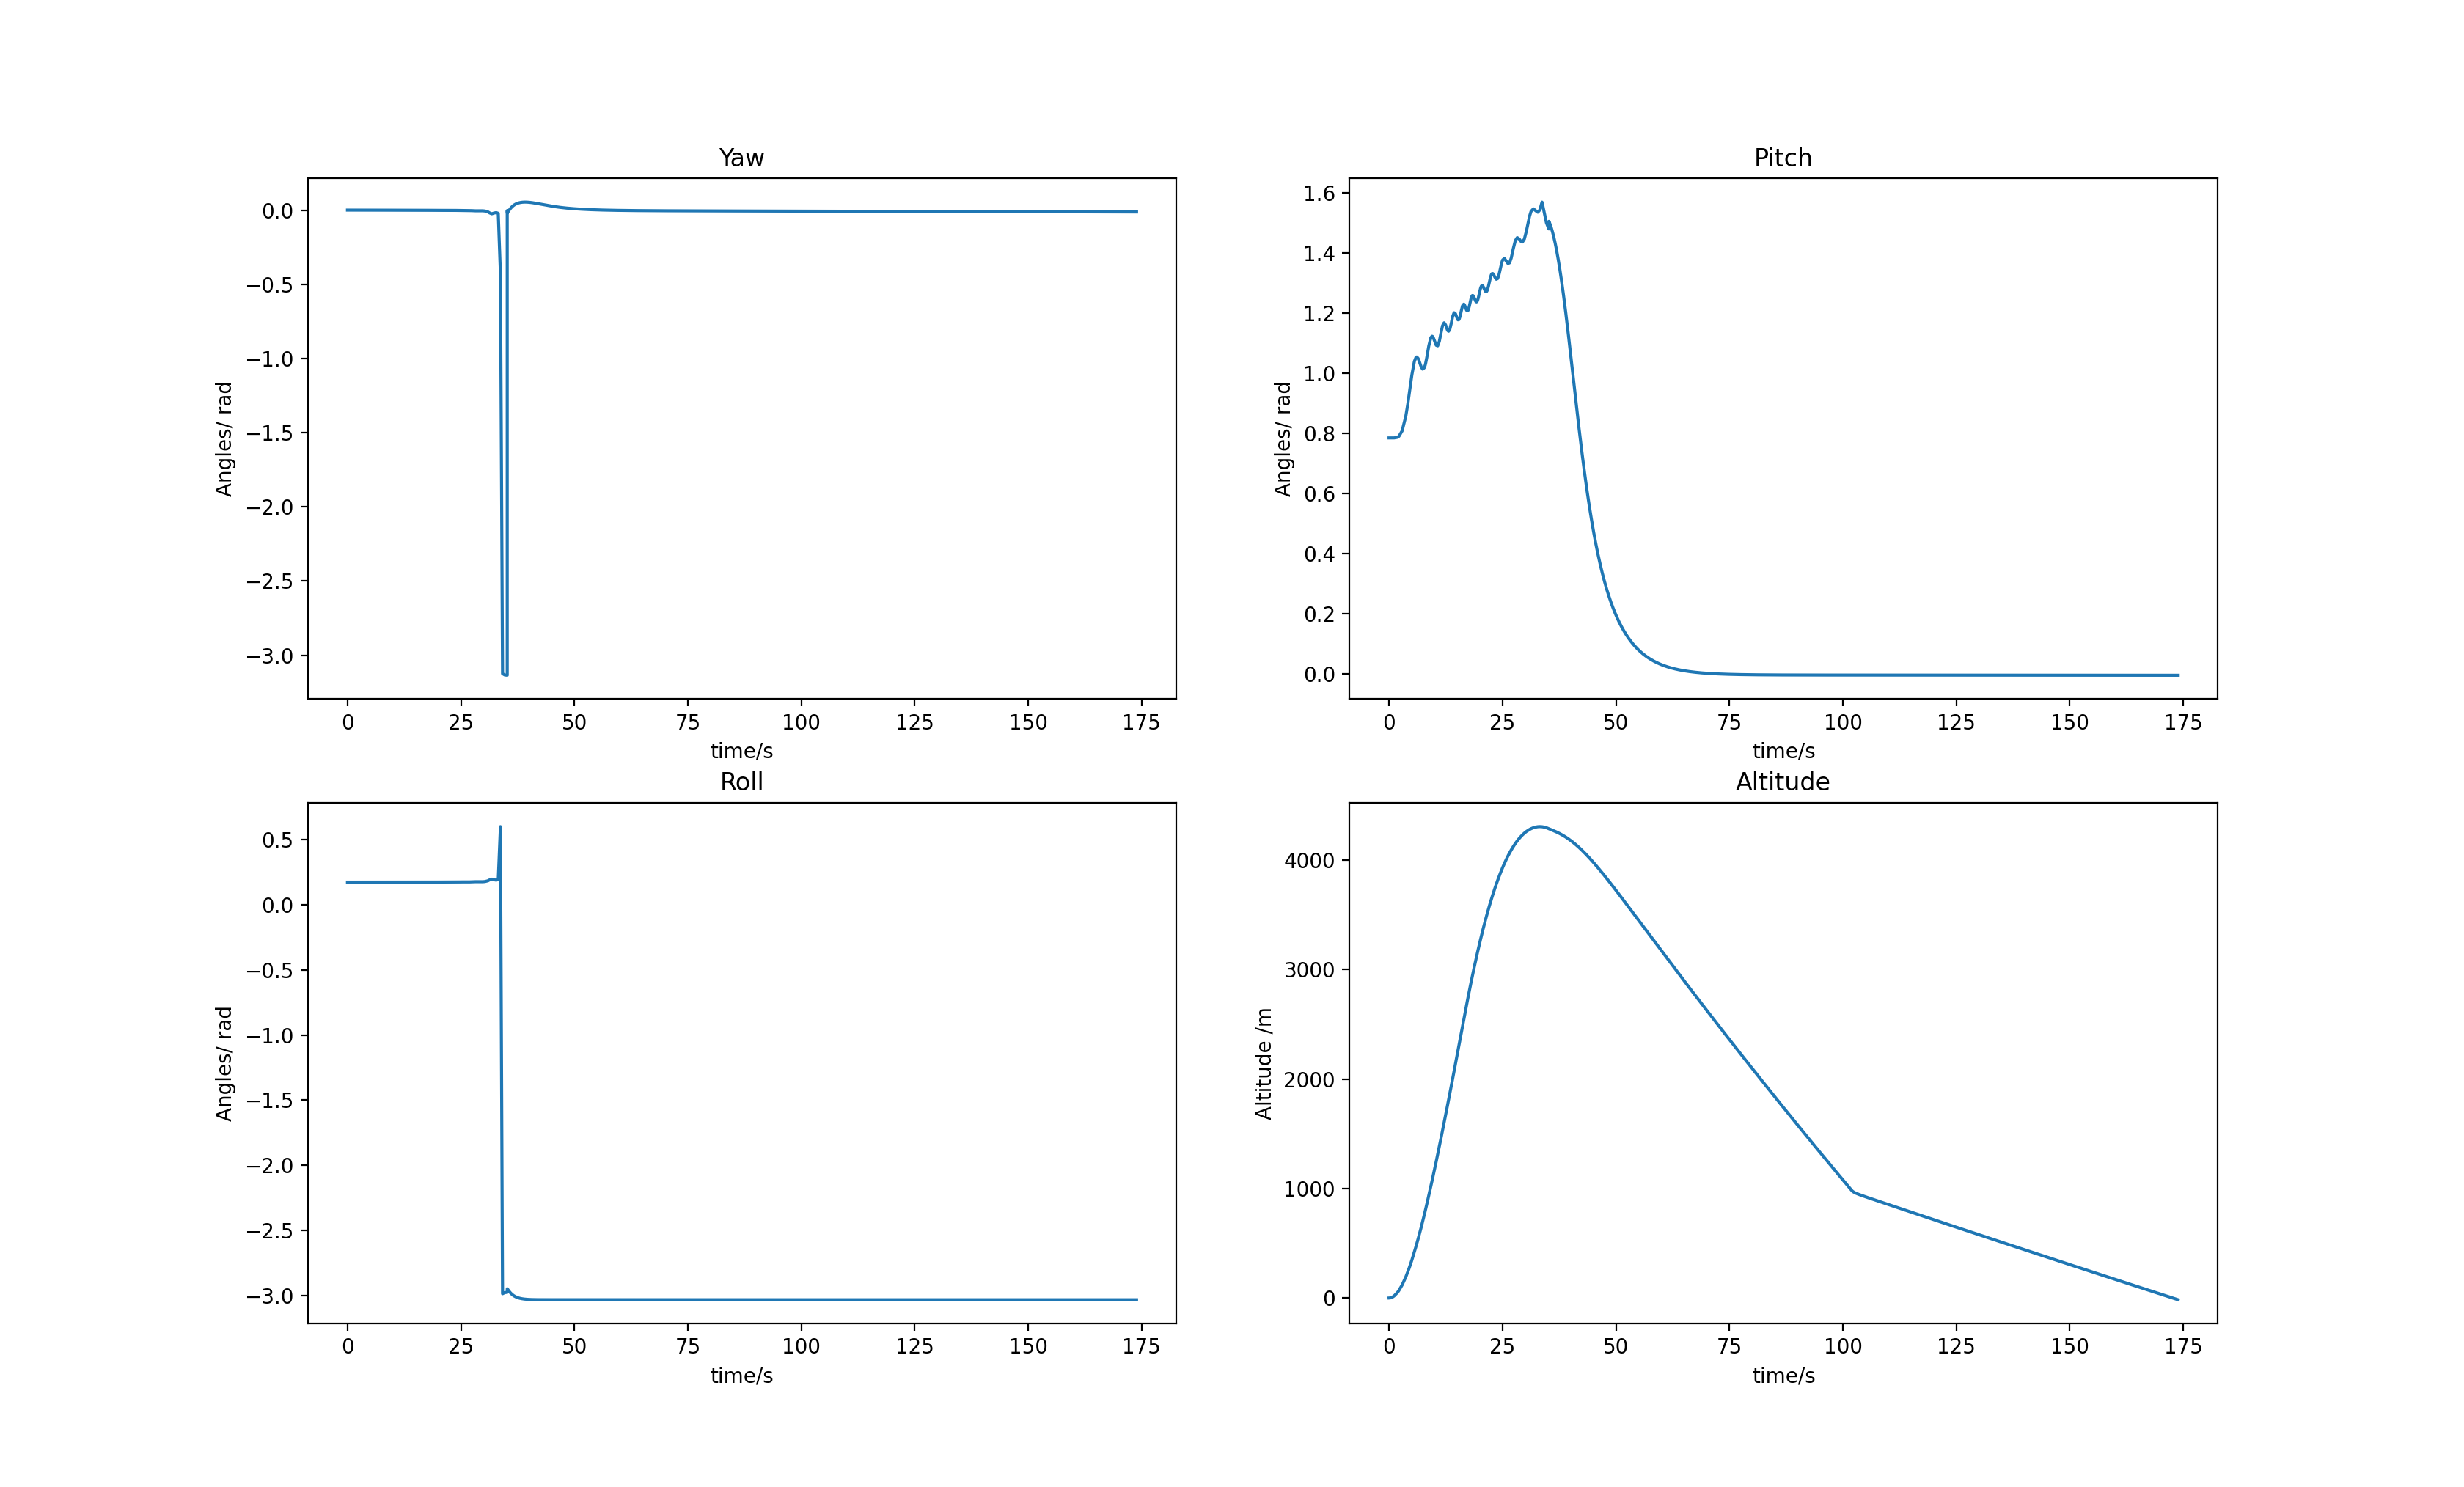
\includegraphics[width=0.85\textwidth]{images/example3b.png}
    \end{frame}
    \begin{frame}
        \frametitle{Monte Carlo Analysis}
        \framesubtitle{What is that}
        \begin{itemize}
            \item Monte Carlo allows you to analyse the effects of variations on a highly non linear system
            \item Essentially randomly generating variations/error in the input parameters (e.g. thrust, drag coefficients, rail angle)
            \item Possible to calculate errors/confidence intervals for predicted trajectories (maths of this is yet to come)
        \end{itemize} 
    \end{frame}
    \begin{frame}
        \frametitle{Monte Carlo Analysis}
        \framesubtitle{No rail angle or wind, 1000 itterations}
        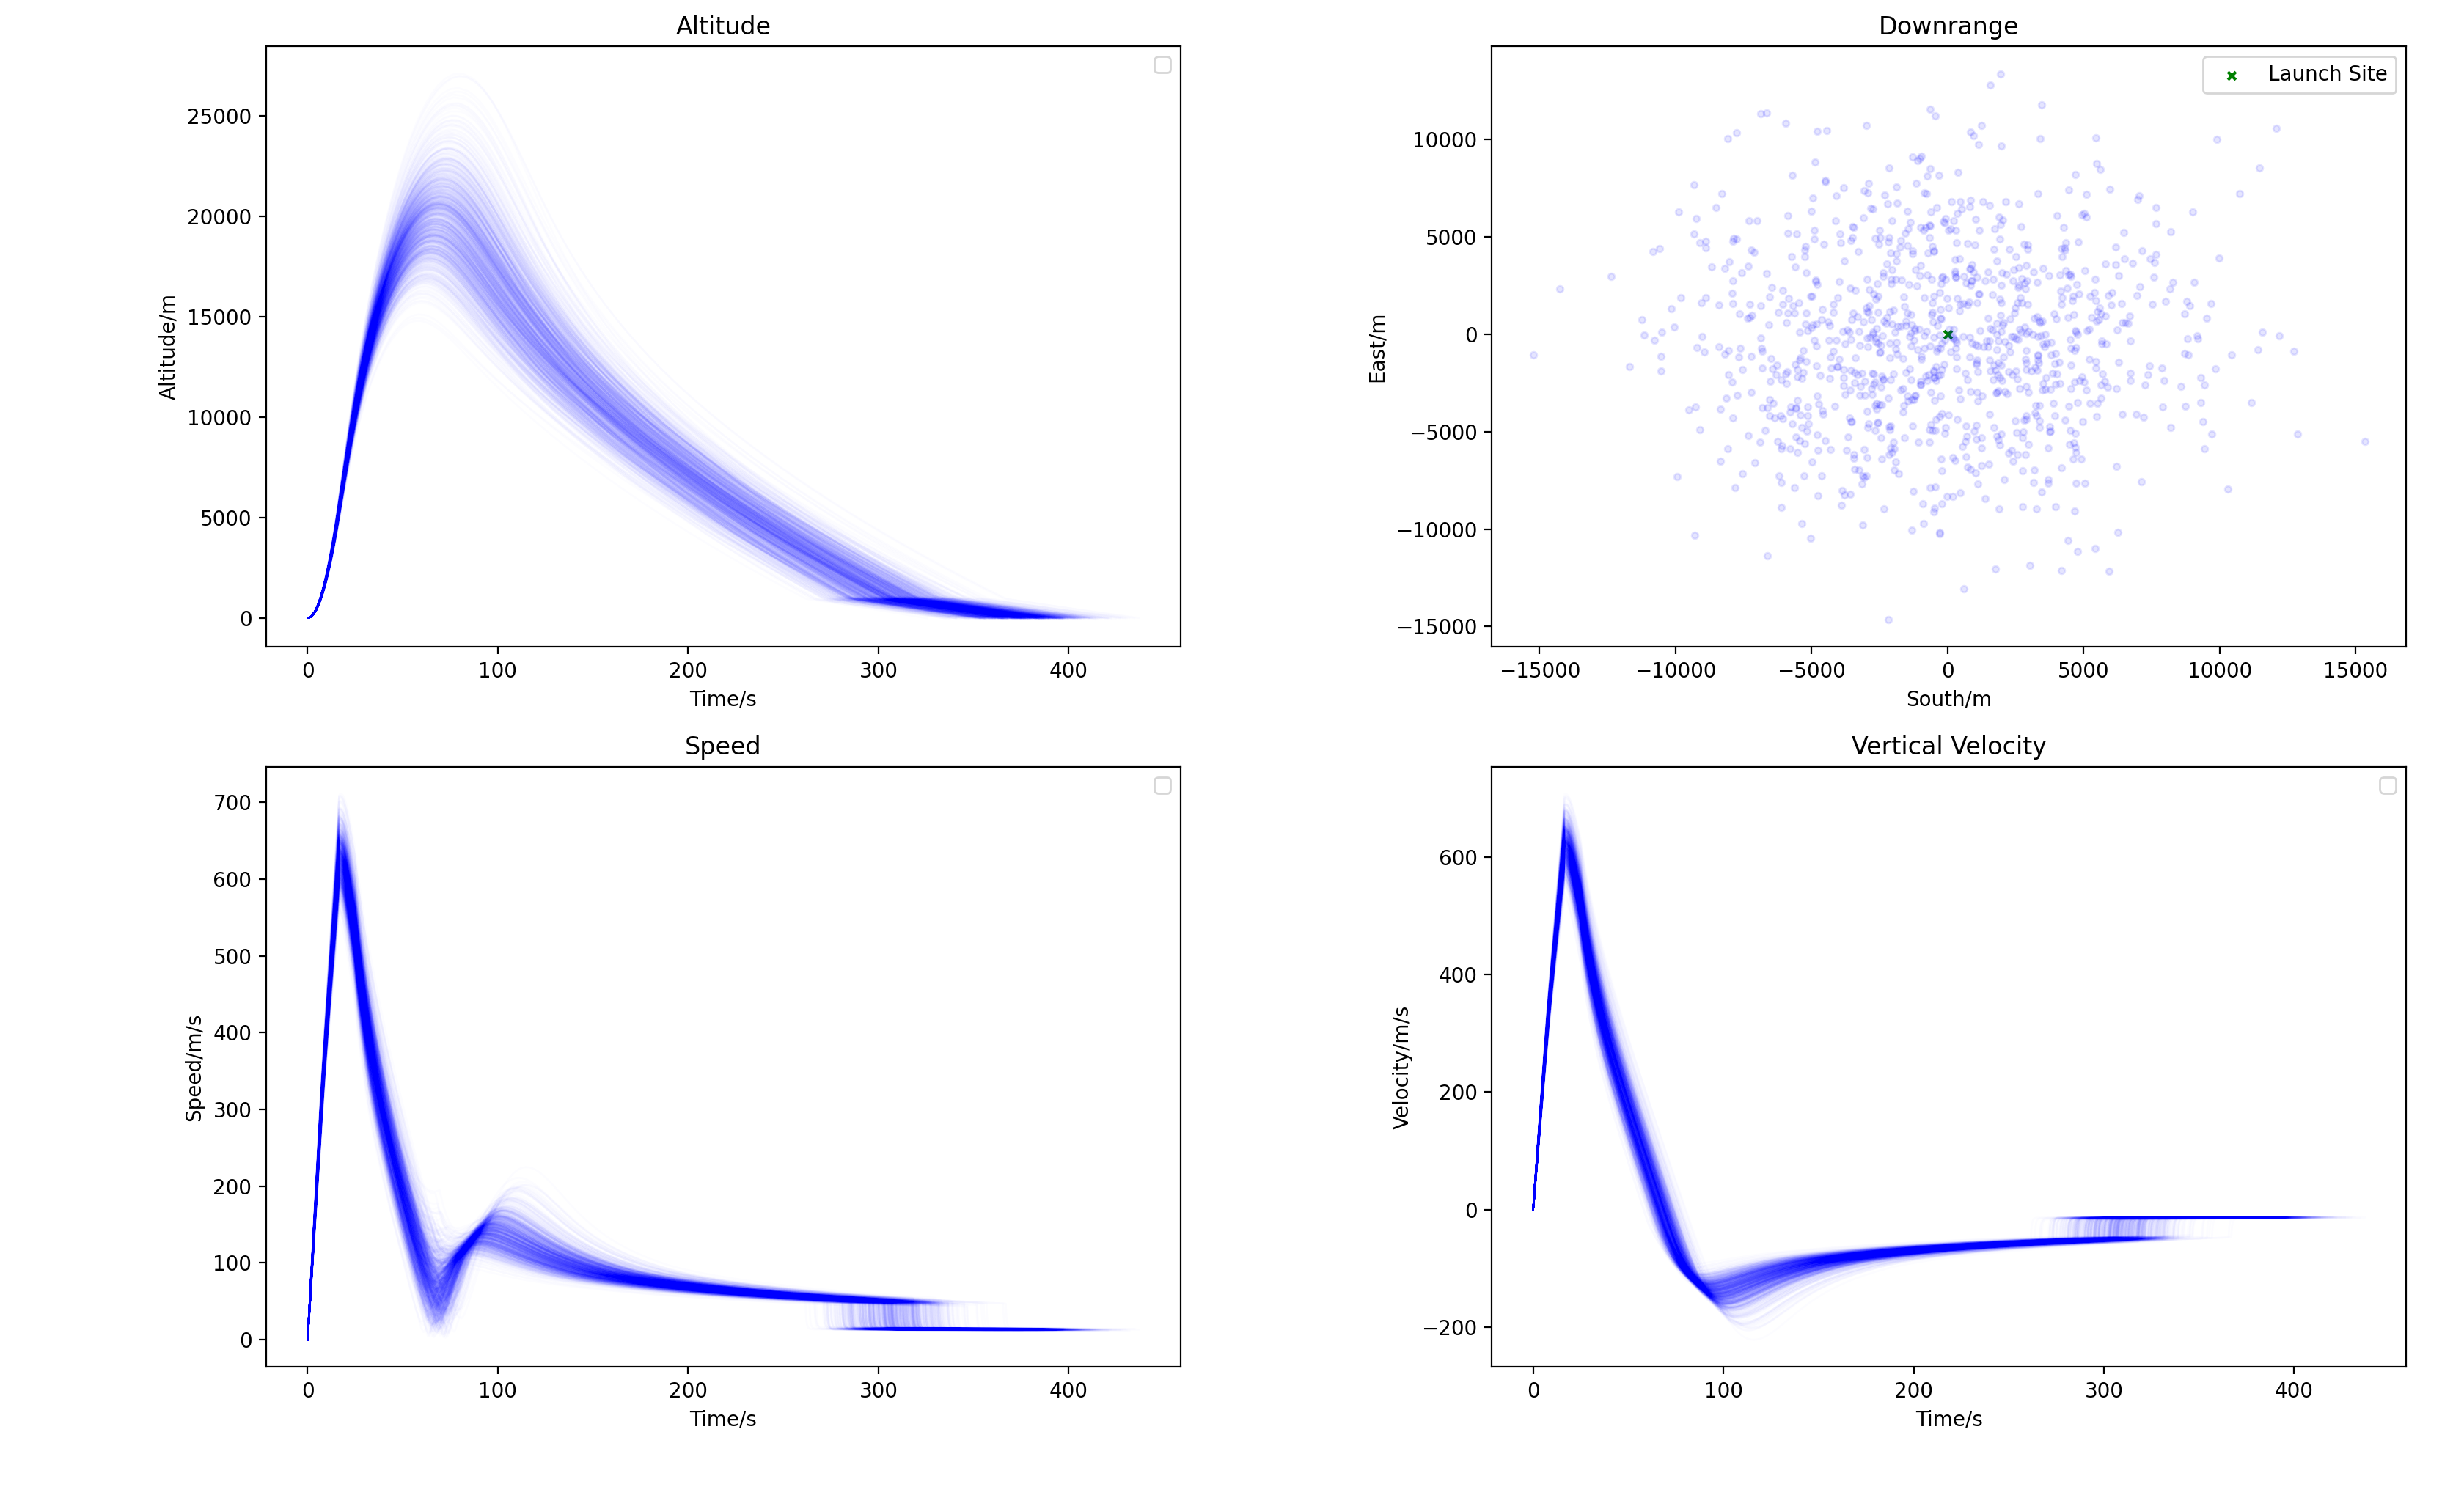
\includegraphics[width=0.85\textwidth]{images/stats_example1.png}
    \end{frame}
    \begin{frame}
        \frametitle{Monte Carlo Analysis}
        \framesubtitle{No rail angle or wind, 1000 itterations}
        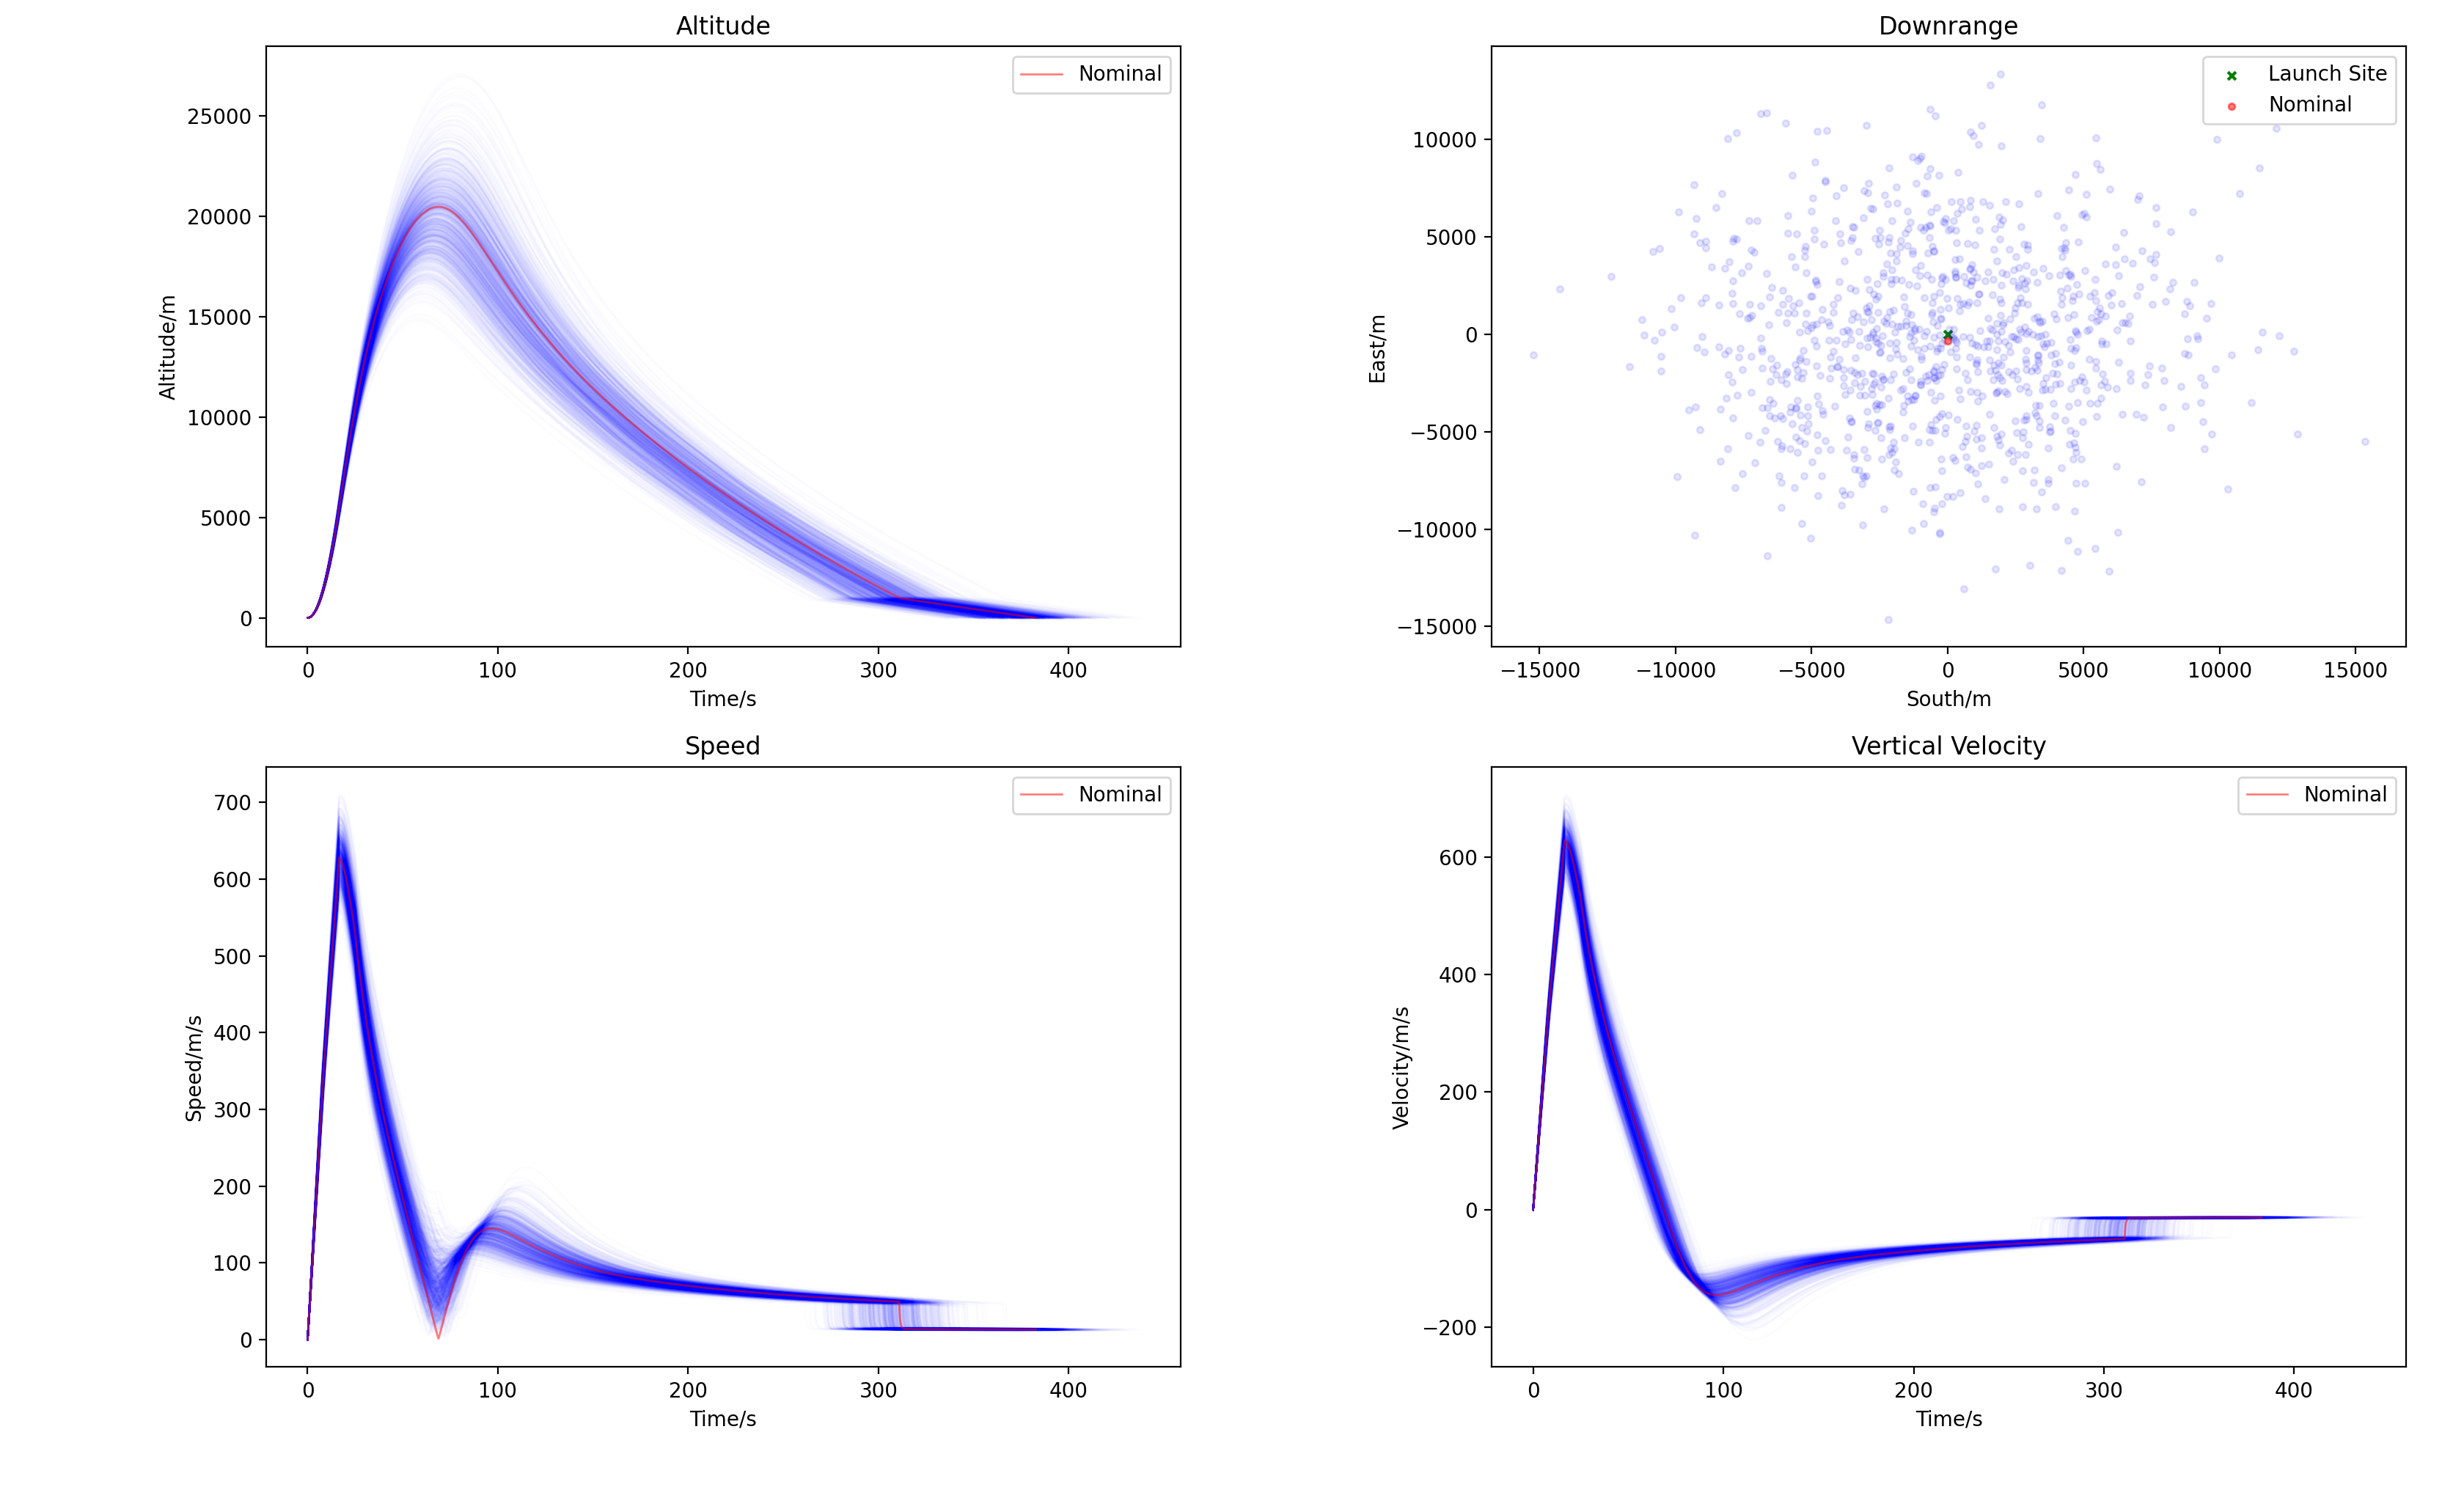
\includegraphics[width=0.85\textwidth]{images/stats_example1_with_nom.png}
    \end{frame}
    \begin{frame}
        \frametitle{Monte Carlo Analysis}
        \framesubtitle{No rail angle or wind, 1000 itterations}
        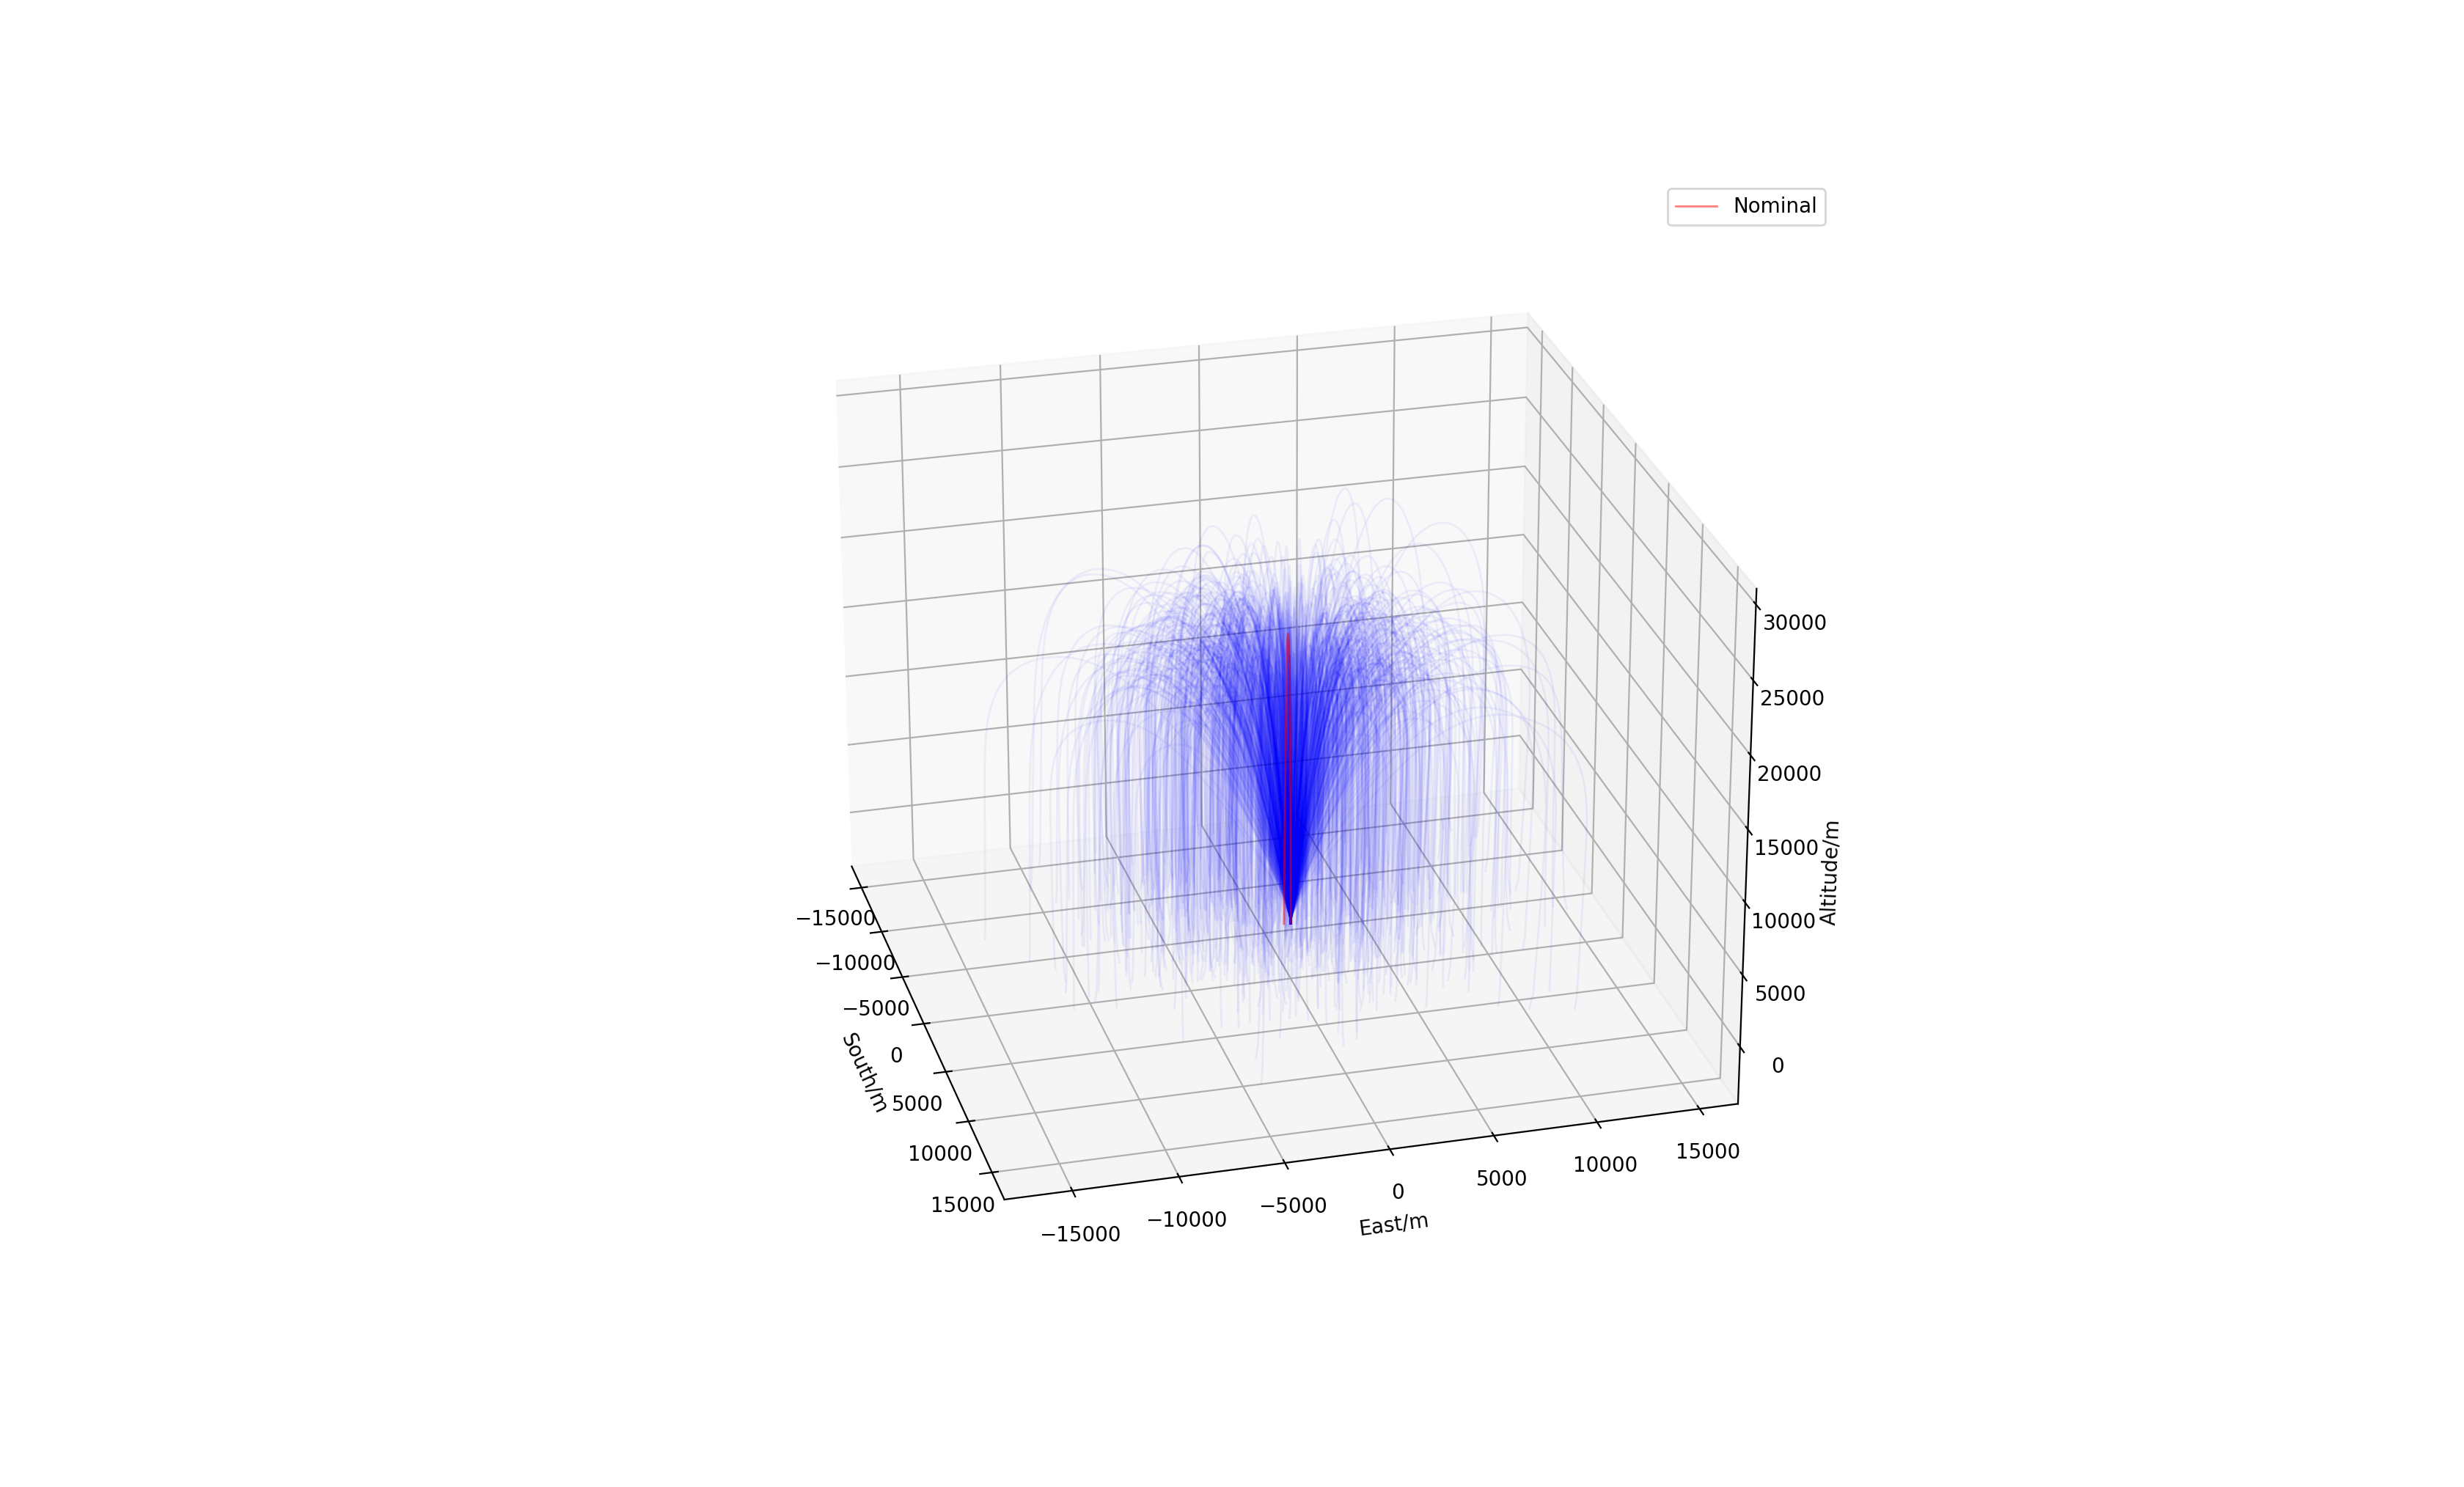
\includegraphics[width=0.85\textwidth]{images/stats_example2_with_nom.png}
    \end{frame}

    \begin{frame}
        \frametitle{Final Notes}
        \framesubtitle{What we have left}
        \begin{itemize}
            \item Proper analysis of the Monte Carlo Results
            \item New more accurate mass model (we currently just have a cylinder)
            \item Better aero model (i.e. including damping etc.)
            \item Aerodynamic heating analysis
            \item Slosh modeling
            \item Couple with CFD for more accurate results 
            \item Finish documentation
            \item Think of a name
        \end{itemize} 
    \end{frame}
\end{document}